% !TeX program = pdflatex

\documentclass[10pt,%                      % corpo del font principale
               b5paper,%                   % carta A4
               twoside,openright,%         % fronte-retro
               % oneside,openany,%         % solo fronte
               titlepage,%                 % frontespizio
               headinclude,,footinclude,%  % testatina e piede di pagina
               cleardoublepage=empty,%     % pagine vuote senza testatina e piede di pagina
               captions=tableheading,%     % didascalie in cima alle tabelle
               ]{scrbook}                  % book class of KOMA-Script;
               
% packages and style
\usepackage{styles/preamble}
% personal settings
\usepackage{styles/settings}    
% bibliography
\addbibresource{bibliography/particle.bib}
\addbibresource{bibliography/qml.bib}
\addbibresource{bibliography/ml.bib}
\addbibresource{bibliography/quantumcomputing.bib}




\begin{document}
    \pagestyle{scrheadings}

    %******************************************************************
    % Front Matter
    %******************************************************************
    % !TeX root = ../../main.tex

\pdfbookmark{Cover}{Cover}
\newgeometry{width=370pt,height=650pt,centering}

\begin{center}
	
\includegraphics[width=11cm]{logos/uni.jpg}
	\vspace*{10pt}

	Laurea Magistrale in Fisica\\
	\myDepartment\\
	\vspace*{5pt}

	\vfill

	{\Huge \myTitle}\\
    \vspace*{30pt}

	\vfill

	\textbf{Supervisor:} \hfill \textbf{Candidate:}\\
	\myProf \hfill \myName\\
    \begin{flushleft}
    \textbf{Co-Supervisor:} \\
    \cosupervisor \\
    \cocosupervisor \\
    \end{flushleft}
	\vspace*{15pt}
	Anno Accademico 2023/2024
\end{center}
	
	
\pagenumbering{gobble}

\cleardoublepage
\restoregeometry
    \pagenumbering{roman}

    \cleardoublepage
    %\section*{Ringraziamenti}

Innanzitutto ci tengo a ringraziare il professor Stefano Carrazza per avermi accolto nella collaborazione Qibo, 
per avermi proposto un progetto di tesi molto stimolante e per la straordinaria esperienza al CERN.\\
Inoltre ci tengo a ringraziare il professor Carrazza per i numerosi suggerimenti che mi ha fornito durante tutto 
il lavoro della mia tesi.\\
Durante quest’anno mi sono sentito molto felice di esser parte della comunità di Qibo, perché mi sono sentito 
parte di una collaborazione dinamica, ricca di stimoli e colma di persone preparatissime.
Per queste ragioni mi sono subito fidato del progetto di tesi che mi è stato proposto perché ero certo di 
essere in buone mani.\\
L’esperienza al CERN è stata tanto inaspettata quanto apprezzata. Ho avuto l’occasione unica di parlare 
e conoscere giovani aspiranti fisici provenienti da tutto il mondo; ho avuto l’occasione di seguire le 
lezioni di professori di fama internazionale, che hanno ulteriormente accresciuto la mia passione per la Fisica.\\
Ci tengo anche a ringraziare Matteo che è sempre stato disponibile durante tutto quest’anno, che mi ha 
aiutato a dare una una forma ed una struttura alle mie idee e a farle diventare una tesi della quale sono 
soddisfatto.\\
Ci tengo anche a ringraziarlo per il supporto, per i consigli e per il tempo passato insieme al CERN questa estate.\\

Ci tengo a ringraziare la mia famiglia, nella cui unità non smetto mai di credere.
Ringrazio i miei genitori per avermi dato una educazione non convenzionale.\\

Ci tengo a ringraziare i miei amici che sono la parte più bella della mia vita. Sto scrivendo questo cappello 
introduttivo, dopo avervi ringraziato singolarmente e solo ora che mi sono preso del tempo per riflettere 
sul rapporto che ho con ciascuno di voi mi rendo conto di quanto bene vi voglia e di quanto siate importanti per me. 
Negli ultimi anni lo studio mi ha catturato e spesso ho avuto la sensazione di trascurare alcune delle mie amicizie, 
ma voglio ringraziarvi per la pazienza e la comprensione che avete avuto.\\

Ringrazio Lisbo per le fantastiche cene, per le partite del Milan e per le storie divertenti che ci hai raccontato.\\
Ringrazio Ripo per le foto che anno immortalato tutte le nostre vacanze, per le cene in via Lario, per le storie 
dei tuoi studenti e per quella giornata divertente a casa dei tuoi parenti in Abruzzo.\\
Ringrazio Bigno per essere il collante del nostro gruppo (non vedo l’ora di esplorare Pavia insieme!). 
Senza di te il gruppo non sarebbe unito e amalgamato.\\
Ringrazio Zolo per le sue buffe smorfie e per la sua compagnia silenziosa. \\
Ringrazio Senne e Viktor per la nostra amicizia che resiste la distanza. \\
Ringrazio Anna per le domande divertenti con le quali ci intrattiene in vacanza ogni anno e per aver fondato 
lo “Sleepover Club”, del quale sono fiero di esser parte.\\
Ringrazio la Maddi per avermi mostrato scampoli di Bologna, per volermi bene e per il tempo passato insieme 
durante le nostre vacanze estive.\\
Ringrazio Pelle per la nostra condivisa passione per il cocco, per la cucina alla Wellington, e per tutte le 
serate passate insieme a casa di Mambo.\\
Ti ringrazio anche per le tue battute sagaci e pungenti, e per tutte le cose di geopolitica che mi hai insegnato.\\
Ringrazio Alice per le serate a Ginevra, nelle quali mi sono divertito molto. Sono molto contento che sei 
diventata parte del nostro gruppo di amici, la tua solarità è apprezzata da tutti.\\
Ringrazio Alice, Alia e Lauren per le gite, le serate e il tempo passato insieme questa estate.
In particolare ci tengo a ringraziare Alia per le nostre serate sotto la pioggia e per le nostre conversazioni, 
che sono state una finestra su un mondo che non conoscevo.\\
Ringrazio Ammar per le lunghe e interessanti conversazioni, per avermi insegnato moltissimo sulla sua cultura e 
per avermi fatto divertire con le sue storie.\\
Ringrazio Fidaa per avermi raccontato una parte del mondo che non conoscevo, per essersi presa a cuore tutti i 
miei problemi, per la sua vitalità contagiosa.
Fidaa sei una persona con un animo buono e coraggioso, e non vedo l’ora di scoprire dove la tua resilienza e 
determinazione ti porteranno.\\
Ringrazio Dosha per essere un cavallo pazzo. Ti ringrazio per tutte le nostre conversazioni stimolanti, per 
avermi accolto nei Galli Cedroni e per le vacanze trascorse insieme.\\
Ringrazio Giulio per essere stato un amico e un confidente, per le sue storie intriganti, per avermi introdotto 
al mondo dei banchetti.\\
Ringrazio Tommi per le partite di calcetto, per i numerosissimi passaggi in auto, ma soprattutto per averci 
ospitato per tre mesi indimenticabili a Baceno.
Porterò quell’esperienza sempre nel cuore.\\
Ringrazio Chiara S. per volermi sempre molto bene e per i mesi trascorsi a Baceno.\\
Ringrazio Chiara D. per le nostre conversazioni e per avermi supportato durante questi anni.\\
Ringrazio Chiara M. per le nostre conversazioni introspettive e per essere sempre presente e interessata alla mia 
vita nonostante la distanza che ci separa.\\
Ringrazio Dave per essere stato al mio fianco durante tutto il percorso universitario, per avermi supportato 
e motivato anche nei momenti in cui vacillavo. Ti ringrazio anche per avermi fatto assaggiare cibi stranissimi, 
che in nessun altro luogo del mondo potrei trovare. Tutti i bellissimi momenti che abbiamo passato insieme in 
questi anni rimarranno sempre impressi nella mia memoria, fra questi ne menziono solo alcuni: le partitelle a 
Plesios, la grigliata a Plesios, la vacanza a Casasco, le giornate sulla neve, le finali NBA …\\
Ringrazio Luca per essere (insieme a Bigno) il collante del nostro gruppo. La tua presenza è fondamentale per 
il benessere di tutti durante le nostre uscite, durante le nostre vacanze. Vederti e parlare con te mi mette 
sempre di buon umore. Non dimenticherò mai la quantità di zucchero che mettevi nel te’ a Baceno, non dimenticherò 
mai lo scherzo che ti abbiamo fatto in Toscana. Ti ringrazio Luca per sopportare tutte le mie domande pungenti di 
storia e geopolitica, sei per me un pozzo senza fondo di informazioni interessantissime.\\
Ringrazio Edo per tutte le nostre conversazioni, che sono state un vero arricchimento e occasione di crescita.
Parlare con Edo è sempre un piacere, perché ogni frase di uno si incastra con una frase dell’altro componendo un 
nuovo e inaspettato ragionamento, che ci porta sempre a scoprire e a comprendere qualcosa di nuovo sul mondo che ci circonda. 
Ti ringrazio anche per tutti gli elogi con i quali mi hai aiutato ad abbattere le mie insicurezze.
Il tempo che abbiamo passato insieme in questi anni è indimenticabile e importantissimo per me: Napoli, le 
mattinate in Bicocca, la vacanza silenziosa a Varzo, …\\
Grazie davvero Edo.\\
Ringrazio Pleba per la nostra longeva amicizia. La nostra amicizia è indissolubile e non riesco ad immaginarmi 
una vita nella quale non siamo amici. Ti ringrazio per volermi bene, per supportarmi, per motivarmi e stimolarmi 
da più di 10 anni. Ti ringrazio per essere stato un amico vero sin dall’inizio del liceo. Nessuno ha seguito la 
mia evoluzione e la mia crescita con il tuo interesse e la tua vicinanza. Hai sempre avuto a cuore tutte le cose 
che mi hanno riguardato nel corso degli anni come se ti riguardassero direttamente.
Hai vissuto le mie vittorie come fossero tue e per questo ti sarò sempre grato. Ripercorrere tutto quello che 
abbiamo vissuto insieme sarebbe impossibile, ma ci tengo a menzionare qualche episodio divertente: i votacci in 
condotta, le grigliate e pizzate a Varazze, i tornei di calcio di fine anno, le finali NBA, i superbowl, il 
fantacalcio, le recensioni di tutti i bar di Milano, la gita a Berlino, la gita ad Assisi, …\\
Ringrazio Mambo per la nostra amicizia indissolubile. Sin dal liceo sei stato per me un esempio da seguire e un 
modello a cui ispirarmi.
Sei un punto di riferimento. Prima gli Scriddy, poi il gruppo del Milan e infine i Cavers: i nostri gruppi di 
amici cambiano nome, ma la nostra amicizia è una costante. Potrei scrivere una lista lunghissima di episodi 
indimenticabili che abbiamo vissuto insieme, ma mi limiterò a citarne qualcuno: ascoltare la musica di Frah 
Quintale su un letto matrimoniale in vacanza, i Galli Cedroni, il rito di iniziazione Scriddy, le partite a 
Risiko mangiando i pancake della Tere, le serate a vedere il Milan, …
Non potrò mai ringraziarti abbastanza 
per il supporto incondizionato	che mi hai dato quest’anno. Questi mesi che ho trascorso a casa tua sono stati 
sicuramente fra i più belli del mio percorso universitario. \\
Grazie Mambo. \\

Dopo aver ringraziato i miei amici ci tengo a ringraziare la persona più importante della mia vita. 
Faccio fatica a trovare le parole per 
esprimere l’amore e la gratitudine che provo nei tuoi confronti.
In questi anni il nostro rapporto è evoluto e maturato in modo naturale, come il fluire di un fiume, e oggi, 
a pochi giorni dal trasloco nella nostra prima casa, mi emoziona ripensare al giorno in cui ci siamo conosciuti.
Ricordo ancora nitidamente quella serata al planetario. Sei stata l’imprevisto più bello di questi due anni di 
studi magistrali.
Ti ringrazio per volermi bene, per sopportarmi e supportarmi. 
Non so come avrei fatto senza di te in questi anni.
Grazie Cecilia.\\

Infine ci tengo a ringraziare me stesso.\\ 
Questi anni sono stati impegnativi e troppo spesso ho screditato i miei successi.
Voglio elogiare la mia resilienza, la mia costanza, la mia tenacia e la mia determinazione.
Voglio ringraziare il giovane Niccolò, che è riuscito a superare in modo eccellente ogni esame, nonostante le 
attanaglianti insicurezze.\\
Durante questi anni ho affrontato ogni esame con lo scopo di voler dimostrare agli altri e a 
me stesso di essere in grado di superare qualsiasi tipo di ostacolo si presentasse nel mio cammino.
La paura di fallire mi ha ostacolato e non mi ha permesso di ragionare e studiare nel pieno delle mie possibilità.
D'ora in avanti questo paradigma cambierà, non ho più nulla da dimostrare a nessuno.\\
Il paradigma che muoverà le mie scelte sarà quello della curiosità e del piacere di imparare.\\

Per ultima ci tengo a ringraziare la Fisica, per aver dato un senso alle mie giornate negli ultimi sei anni.\\
Mi sono iscritto a questo percorso di studi senza particolari motivazioni, se non un vago e mal definito sentimento 
di rivalsa nei confronti delle materie che avevano maggiormente ostacolato i miei studi liceali.\\
Oggi e per sempre sarò grato a quella scelta poco ponderata.\\


    \pagestyle{scrheadings} 
    %*******************************************************
% Contents
%*******************************************************
\phantomsection
\pdfbookmark{\contentsname}{tableofcontents}
\setcounter{tocdepth}{2}
\begingroup 
    \let\clearpage\relax
    \let\cleardoublepage\relax

    \tableofcontents
\endgroup
\markboth{\spacedlowsmallcaps{\contentsname}}{\spacedlowsmallcaps{\contentsname}} 

\begingroup 
    \let\clearpage\relax
    \let\cleardoublepage\relax
\endgroup
    \cleardoublepage
    \pagenumbering{arabic}
    
\chapter{Quantum Information Theory}

Quantum Information Theory is the field that studies how quantum systems can be used to represent, process, and transmit information.
Such quantum systems - atoms, ions, light modes, superconducting systems - can be in superpositions and can feature entanglement, 
and the fundamental idea is that by taking advantage of these quantum properties we can come up with new ways of representing, processing
and transmitting information.\\
Quantum Information Theory has many different subfields:

\begin{itemize}
    \item \textbf{Quantum key distribution}.\\
    Quantum key distribution allows to transmit classical information from one place to another.
    The basic idea at the heart of quantum key distribution is that one cannot learn a quantum state without to some extent disturbing it.
    This field is not a far-fetched dream, but it is already a reality: companies like IDQuantique are already providing quantum-based encryption 
    services for secure communications.
    \item \textbf{Quantum Metrology}.\\
    Quantum Metrology aims to improve the accuracy in certain sensing and metrology tasks.
    \item \textbf{Quantum Simulation}.\\
    The main idea of Quantum Simulation is that if we aim to simulate a certain quantum systems we better use a quantum systems that we can
    control and manipulate.
    It is possible to distinguish to branches in quantum simulation: \textit{analog quantum simulators}, where
    one basically reconstructs a given Hamiltonian under precisely controlled conditions; \textit{digital quantum simulators}, which can 
    be seen as basically quantum computers that perform Hamiltonian simulation.
    \item \textbf{Quantum Computing}.\\
    The most prominent and exciting subfield of Quantum Information Theory is Quantum Computing. This area focuses on developing quantum computers, 
    which use single quantum systems - qubits - as the basic unit of information, replacing the classical bits used in traditional computers.\\
    Numerous algorithms that take advantage of a quantum computer - quantum algorithms - have been developed and have shown \textit{quantum advantage},
    which means that they outperform (in computational complexity) classical computer when performing a certain task.
    Examples include Shor's factorization algorithm, which finds the factors \textit{a} and \textit{b} of a product \textit{ab} where 
    \textit{a} and \textit{b} are prime numbers, and Grover's algorithm, which searches for an element in an unstructured database.\\
    There are various models for implementing quantum computation: gate-based (or circuit-based) quantum computation, measurement-based (or one-way) 
    quantum computation, adiabatic quantum computation, annealing quantum computation.
\end{itemize}

The following sections will briefly discuss the postulates of Quantum Mechanics (for both \textit{isolated quantum system} and 
\textit{open quantum system}) and elements of Quantum Computing (circuit-based quantum computation, measurement-based quantum computation).\\
For further informations on this topic \cite{Paris_2012}.

\section{Postulates of Quantum Mechanics}

Quantum Mechanics has three postulates.\\
Each postulate of quantum mechanics has two distinct versions, depending on whether we are considering an 
\textit{isolated quantum system} (I) or an \textit{open quantum system} (O).

\paragraph{Postulate 1 – States of a quantum system}
\begin{enumerate}
    \renewcommand{\labelenumi}{I)}
    \item Each physical system is associated to an Hilbert space $\mathcal{H}$. The possible states of the quantum system are 
    normalized vectors $|\psi \rangle \in \mathcal{H}$.
    A composite physical system is associated to a Fock space which is the tensor product of multiple Hilbert space (one for each subsiystem):
    $\mathcal{H} = \mathcal{H}_1 \otimes \mathcal{H}_2 \otimes ... \otimes \mathcal{H}_n$
    \renewcommand{\labelenumi}{O)}
    \item Each physical system is associated to an Hilbert space $\mathcal{H}$. 
    The possible states of the quantum system are represented by a density matrix $\rho$, which has the following charateristics:
    \begin{align}
        \rho = \rho^{\dagger}
        \qquad
        tr(\rho) = 1
        \qquad
        \rho \ge 0
    \end{align}
\end{enumerate}

The main difference between the two postulates is that an isolated quantum system does not interact with its environment and thus remains 
in a pure state. In contrast, an open quantum system interacts with its environment, leading to a situation where the system can be in a 
mixed state, described by a density matrix that accounts for various possible states and their associated probabilities.

\begin{align}
    \{p_k, |\psi_k \rangle \}
    \qquad 
    \sum_k p_k = 1
\end{align}


\paragraph{Postulate 2 – Quantum measurements}
\begin{enumerate}
    \renewcommand{\labelenumi}{I)}
    \item Observable quantities are described by hermitian operators $\hat{O} = \hat{O}^{\dagger}$.
    The observable O admits a spectral decomposition:
    \begin{equation} 
        \hat{O} = \sum_i O_i |O_i \rangle \langle O_i | = \sum_i O_i \hat{P}_i
    \end{equation} 
    where $O_i$ are real eigenvalues, $\hat{P}_i$ is the projector corresponding to the eigenvalue $O_i$, $|O_i \rangle$ are eigenstates, which are
    a orthonormal basis of the Hilbert space associated to the physical system.\\
    The Born rule states that the probability of obtaining $O_i$ when measuring $\hat{O}$ and the overall expectation value of $\hat{O}$ are:
    \begin{align}
        p(O_i) = tr(|\psi \rangle \langle \psi | \hat{P}_i) 
        \qquad
        \langle \hat{O} \rangle = tr(|\psi \rangle \langle \psi | \hat{O})
    \end{align}


    \renewcommand{\labelenumi}{O)}
    \item Observable quantities are described by hermitian operators $\hat{O} = \hat{O}^{\dagger}$.
    The observable O admits a spectral decomposition:
    \begin{equation} 
        \hat{O} = \sum_i O_i |O_i \rangle \langle O_i | = \sum_i O_i \hat{P}_i
    \end{equation} 
    where $O_i$ are real eigenvalues, $P_i$ is the projection operator corresponding to the eigenvalue $O_i$, $|O_i \rangle$ are eigenstates, which are
    a orthonormal basis of the Hilbert space associated to the physical system.\\
    Given $\rho \in \mathcal{L}(\mathcal{H})$, the probability of measuring y is:

    \begin{equation}
        p_y = tr(\rho \hat{\Pi}_Y)
    \end{equation}
 
    The charateristics that the POVMs $\{\hat{\Pi}_Y\}$ must satisfy for $\{p_y\}$ to be valid probabilities are:

    \begin{align}
        \sum_i \hat{\Pi}_i = \mathds{I}
        \qquad
        \hat{\Pi}_i \ge 0
    \end{align}

\end{enumerate}

The main difference between the two postulates is that $\{\hat{P}_Y\}$ are PVMs (Projection-Valued Measures), whereas $\{\hat{\Pi}_Y\}$ are POVMs
(Positive Operator-Valued Measures).
PVMs are orthogonal and complete, which means they automatically satisfy the properties of projection operators:

\begin{align}
    \hat{P}_i \hat{P}_j = \delta_{ij} \hat{P}_i
    \qquad
    \rightarrow
    \qquad
    \hat{P}_i^2 = \hat{P}_i
\end{align}

The second postulates for isolated quantum systems and open quantum systems are connected by the \textit{Naimark theorem}.

\begin{theorem}[Naimark theorem]
    Given an Hilbert space $\mathcal{H}_A$, for every POVM $\hat{\Pi}_Y \in \mathcal{L}(\mathcal{H}_A)$ it exists an 
    Hilbert space $\mathcal{H}_B$ such that:
    \begin{itemize}
        \item $\exists$ $\rho_B \in \mathcal{L}(\mathcal{H}_B)$
        \item $\exists$ $U \in \mathcal{L}(\mathcal{H}_A \otimes \mathcal{H}_B)$
        \item $\exists$ $\hat{P}_y \in \mathcal{L}(\mathcal{H}_B$)
    \end{itemize}
    Therefore, given $\rho_A \in \mathcal{L}(\mathcal{H}_A)$ the probability of measuring y is:

    \begin{equation}
        p_y = tr_A(\rho_A \hat{\Pi}_Y) = tr_{AB}(U (\rho_A \otimes \rho_B) U^{\dagger}(\mathds{1} \otimes \hat{P}_Y))
    \end{equation}
\end{theorem}

\paragraph{Postulate 3 – Dynamics of a quantum system}.
\begin{enumerate}
    \renewcommand{\labelenumi}{I)}
    \item The dynamical evolution of a physical system from an initial time $t_0$ to a time $t \ge t_0$ is described by a unitary operator 
    $\hat{U}(t, t_0)$.
    If $\psi_{t_0}$ is the state in the inital time $t_0$, then the state at time t is:
    \begin{equation}
        |\psi_t \rangle = \hat{U}(t, t_0) | \psi_{t_0} \rangle
    \end{equation}
    Stone's theorem states that:
    \begin{equation}
        \hat{U}(t, t_0) = exp(\frac{-i}{\hbar} (t-t_0) \hat{H})
    \end{equation}
    where $\hat{H}$ is the hamiltonian that regulates the dynamic of the system.

    \renewcommand{\labelenumi}{O)}
    \item The dynamical evolution of a physical system from an initial time $t_0$ to a time $t \ge t_0$ is described by a quantum dynamical map $\varepsilon$:
    
    \begin{align}
        \varepsilon : \mathcal{L}(\mathcal{H}) &\rightarrow \mathcal{L}(\mathcal{H}) \\
        \rho &\mapsto \varepsilon(\rho) \\
    \end{align}

    A quantum dynamical map has the following charateristics:
    \begin{itemize}
        \item Positive: $\varepsilon(\rho) \ge 0$ $\forall \rho$;
        \item Trace preserving: $tr(\rho) = tr(\varepsilon(\rho)) = 1$;
        \item Linear;
        \item Completely positive;
    \end{itemize}
\end{enumerate}

The third postulates for isolated quantum systems and open quantum systems are connected by the \textit{Kraus theorem}.

\begin{theorem}[Kraus theorem]
    Given an Hilbert space $\mathcal{H}_A$ and a density matrix $\rho_A \in \mathcal{L}(\mathcal{H}_A)$, $\varepsilon$ is a quantum dynamical map if and 
    only if $\varepsilon$ can be expressed as:

\begin{equation}
    \varepsilon(\rho_A) = \sum_i M_i \rho_A M_i^{\dagger} 
\end{equation}

such that $\sum_i M_i M_i = \mathds{1}$.
Moreover $\varepsilon$ is a quantum dynamical map if and only if it exists an Hilbert space $\mathcal{H}_B$, a density matrix 
$\rho_B \in \mathcal{L}(\mathcal{H}_B)$ and a unitary matrix $U \in \mathcal{L}(\mathcal{H}_A \otimes \mathcal{H}_B)$ such that:

\begin{equation}
    \varepsilon(\rho_A) = tr_B(U(\rho_A \otimes \rho_B)U^{\dagger})
\end{equation}


\end{theorem}



\section{Quantum Computing}

\textit{Quantum Computing} is one of the subfields of Quantum Information Theory.\\
It studies how quantum systems can be used to process information and perform computations.
The basic element of Quantum Computing (and more in general of Quantum Information Theory) is called \textit{qubit}, which describes a two-level quantum 
system, for example a particle having access to the ground state and first excited state of an energy potential or the two polarization states of a photon.
Independently of its actual physical realisation, the quantum state of a qubit is mathematically described as a vector living 
in a two-dimensional vector space over the complex numbers, namely $\mathcal{C}^2$.


\subsection{Qubits}

A Hilbert space is a complete inner product space over the field of complex numbers.
Some examples of Hilbert spaces are:

\begin{enumerate}
    \item The linear space $\mathcal{C}^n$ is a Hilbert space with the scalar product:

\begin{equation}
    \langle z , w \rangle = \sum_i \bar{z}_i w_i
\end{equation}

    \item The complex matrices $\mathcal{C}^n \times \mathcal{C}^n$ is a Hilbert space with the Schmidt inner product:

\begin{equation}
    \langle A , B \rangle = tr(A^{\dagger}B)
\end{equation}

\end{enumerate}

A \textit{qubit} is a vector living in the Hilbert space $\mathcal{H} = \mathcal{C}^2$.
A qubit can be expressed as:

\begin{equation}
    |\psi \rangle = \alpha |0 \rangle +  \beta |1 \rangle
\end{equation}

with $\alpha$, $\beta$ $\in \mathcal{C}$ and $|\alpha|^2 + |\beta|^2 = 1$.
A more convenient rewriting of a qubit, that does not take in consideration a global phase (which cannot be observed), is the following:

\begin{equation}
    |\psi \rangle = \cos(\frac{\theta}{2}) |0 \rangle +  e^{i \phi} \sin(\frac{\theta}{2}) |1 \rangle
\end{equation}


\subsection{Bloch Sphere}

The Bloch Sphere is a very intuitive way of describing a qubit (figure \ref{fig:bloch-sphere}).\\
A qubit can be envisioned as a unitary vector on a unitary sphere with the following association:

\begin{align}
    r = 
    \begin{pmatrix}
        r_x \\
        r_y \\
        r_z \\
    \end{pmatrix}
    = 
    \begin{pmatrix}
        sin(\theta)cos(\phi) \\
        sin(\theta)sin(\phi) \\
        cos(\theta) \\
    \end{pmatrix}
\end{align}

In particular the north and south poles of the Bloch Sphere are:

\begin{align}
    | 0 \rangle \rightarrow 
    \begin{pmatrix}
        0 \\
        0 \\
        1 \\
    \end{pmatrix}
    \qquad
    | 1 \rangle \rightarrow 
    \begin{pmatrix}
        0 \\
        0 \\
        - 1 \\
    \end{pmatrix}
\end{align}

\begin{figure}[h]
    \centering
    \includegraphics[scale=0.75]{sections/chapters/Quantum-Information/Images/bloch.pdf}
    \caption{This is the Bloch sphere.}
    \label{fig:bloch-sphere}
\end{figure}


\subsection{Gate-Based Quantum Computation}

Gate-based (or circuit-based) quantum computation is one of the possible realization of quantum computation.
This paradigm of quantum computation is a method of performing quantum computation by applying a sequence of \textit{quantum gates} to a set of qubits. 
The qubits are initialized in a known state, and the gates are used to manipulate the state of the qubits, encoding the problem and 
performing the computation.

\paragraph*{Gates}

Quantum gates perform operations on qubits.\\
Quantum gates are represented by unitary matrices, which ensures that the operations are reversible.
Some examples of single-qubit gates are:

\begin{itemize}
    \item \textbf{Pauli Gates (X, Y, Z)}.\\
    The Pauli-X gate (also known as the quantum NOT gate) 
    flips the state of a qubit. The Pauli-Y and Pauli-Z gates apply phase shifts.

    \begin{align}
    X = \begin{pmatrix}
        0 & 1 \\
        1 & 0 \\
    \end{pmatrix}
    \qquad
    Y = \begin{pmatrix}
        0 & i \\
        -i & 0 \\
    \end{pmatrix}
    \qquad
    Z = \begin{pmatrix}
        1 & 0 \\
        0 & -1 \\
    \end{pmatrix}
    \end{align}

    \item \textbf{Hadamard}.\\
    The Hadamard gate creates a superposition state from the basis states.
    \begin{align}
        | 0 \rangle \rightarrow \frac{| 0 \rangle + | 1 \rangle}{\sqrt{2}}
        \qquad 
        | 1 \rangle \rightarrow \frac{| 0 \rangle - | 1 \rangle}{\sqrt{2}}
    \end{align}
    \begin{align}
        H = \frac{1}{\sqrt{2}}\begin{pmatrix}
            1 & 1 \\
            -1 & 1 \\
        \end{pmatrix}
    \end{align}    
\end{itemize}

Some examples of multi-qubit gates are:

\begin{itemize}
    \item \textbf{CNOT (Controlled-NOT)}.\\
    It flips the state of a target qubit if the control qubit is in state $| 1 \rangle$.
    Therefore, if the control qubit is the first one:
    \begin{align}
        | 0 \rangle 0 \rangle \rightarrow | 0 \rangle 0 \rangle
        \qquad 
        | 1 \rangle 0 \rangle \rightarrow | 1 \rangle 1 \rangle
        \qquad 
        | 1 \rangle 1 \rangle \rightarrow | 1 \rangle 0 \rangle
    \end{align}
    \begin{align}
        CNOT = \begin{pmatrix}
            1 & 0 & 0 & 0 \\
            0 & 1 & 0 & 0 \\
            0 & 0 & 0 & 1 \\
            0 & 0 & 1 & 0 \\
        \end{pmatrix}
    \end{align}
    \item \textbf{SWAP}.\\
    It swaps the state of two qubits.
    \begin{align}
        S = \begin{pmatrix}
            1 & 0 & 0 & 0 \\
            0 & 0 & 1 & 0 \\
            0 & 1 & 0 & 0 \\
            0 & 0 & 0 & 1 \\
        \end{pmatrix}
    \end{align}
    \item \textbf{CZ (Controlled-Z)}.\\
    It applies a Z gate to the target qubit only when the control qubit is in state $| 1 \rangle$.
    \begin{align}
        CZ = \begin{pmatrix}
            1 & 0 & 0 & 0 \\
            0 & 1 & 0 & 0 \\
            0 & 0 & 1 & 0 \\
            0 & 0 & 0 & -1 \\
        \end{pmatrix}
    \end{align}
\end{itemize}


\paragraph*{Quantum Circuit}

A quantum circuit is a sequence of gates applied to a qubit to perform a computational task.\\
A quantum circuits can be represented with diagrams, which are a very intuitive representation of the sequence of operations
performed on a qubit.
An example of a simple quantum circuit is the following:

\begin{center}
\begin{quantikz}[thin lines]
    \lstick{$\ket{0}$} & \qw & \gate{H} & \qw & \gate{X} & \rstick{$\ket{\psi}$}
\end{quantikz}
\end{center}

This circuit represents the following operations:

\begin{align}
    |0 \rangle
    \qquad
    \rightarrow
    \qquad
    \frac{1}{\sqrt{2}}(|0 \rangle + |1 \rangle)
    \qquad
    \rightarrow
    \qquad
    \frac{1}{\sqrt{2}}(|1 \rangle + |0 \rangle)
\end{align}

\subsection{Measurement-Based Quantum Computation}

Measurement-based quantum computation \cite{Raussendorf_2002} is one of the possible realization of quantum computation.\\
Circuit-based quantum computation works both on quantum and classical computers, whereas measurement-based quantum computation is a paradigm
of computation that can be realized only on a quantum computer.
Another key difference between this two pradigms is that the circuit-based model is reversible or two-way, whereas the measurement-based is 
non-reversible or one-way, because it consists in measuring a quantum system which is a destructive and non-reversible operation in Quantum Mechanics.\\
It can be easily proven that these two models are equivalent.

\paragraph{Workflow}
Let's consider a grid of $n \times k$ qubits as shown in figure~\ref{fig:quantum_grid}.
After preparing the qubits in a \textit{cluster state}, an entangled state, measurement-based quantum computation is performed by individually 
measuring the qubits in each column sequentially, starting from the first column and progressing to the penultimate column. The result of 
the computation is encoded in the last column.\\
To implement a specific algorithm within this measurement-based paradigm, the user can adjust 
both the measurement basis for each qubit and the observables measured on each qubit.

\begin{figure}[ht]
\centering
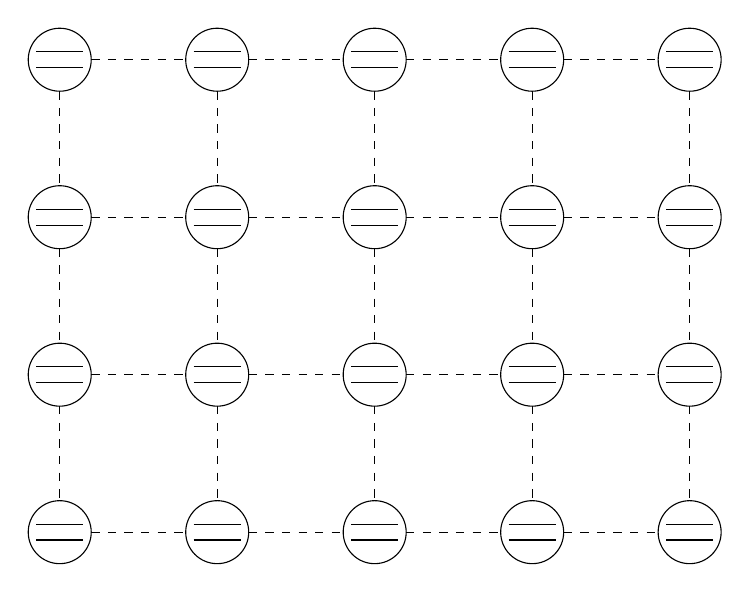
\begin{tikzpicture}
    \def\radius{0.4} % radius of the circles
    \def\dist{2} % distance between the centers of the circles
    \def\lineLength{0.6} % length of the horizontal lines inside the circles
    \def\lineOffset{0.1}

    \foreach \i in {1,2,3,4} {
        \foreach \j in {1,2,3,4,5} {
            \draw (\j*\dist, -\i*\dist) circle (\radius);
            \draw (\j*\dist - \lineLength/2, -\i*\dist + \lineOffset) -- (\j*\dist + \lineLength/2, -\i*\dist + \lineOffset);
            \draw (\j*\dist - \lineLength/2, -\i*\dist - \lineOffset) -- (\j*\dist + \lineLength/2, -\i*\dist - \lineOffset);
        }
    }

    \foreach \i in {1,2,3,4} {
        \foreach \j in {1,2,3,4} {
            \draw[dashed] (\j*\dist + \radius, -\i*\dist) -- (\j*\dist + \dist - \radius, -\i*\dist);
        }
    }
    \foreach \i in {1,2,3} {
    \foreach \j in {1,2,3,4,5} {
        \draw[dashed] (\j*\dist, -\i*\dist - \radius) -- (\j*\dist, -\i*\dist - \dist + \radius);
    }
}

\end{tikzpicture}
\caption{A grid of $5 \times 4$ qubits.}
\label{fig:quantum_grid}
\end{figure}



\subsection{Superconducting Qubits}

Superconducting qubits are one of the many different realization of a quantum computer.\\
In this section I will briefly discuss how it is possible to obtain a two-level system starting from a superconducting circuit.

\paragraph*{LC circuit as an harmonic oscillator}

An LC circuit (figure~\ref{fig:lc_circuit}) is an electric circuit with a capacitor (with capacity C) and an inductor (with inductance L).
By indicating with V the voltage applied to the circuit and with I the current flowing in the circuit, the energy stored in the capacitor and
inductor will be:

\begin{align}
    E_C = \frac{1}{2}CV^2 = \frac{Q^2}{2C}
    \qquad
    E_L = \frac{1}{2}LI^2 = \frac{\phi^2}{2L}
\end{align}

Therefore the energy of the LC circuit will be:

\begin{equation}
    H_{LC} = \frac{Q^2}{2C} + \frac{\phi^2}{2L} = \frac{Q^2}{2C} + \frac{1}{2}C \omega_0^2 \phi^2 
\end{equation}

with $\omega_0 = 1 / \sqrt{LC}$.\\
This is the hamiltonian of an harmonic oscillator with mass C, momentum Q, position $\phi$ and frequency $\omega_0$, hence we can easily quantize
this system by promoting Q and $\phi$ to quantum operators:

\begin{align}
    \hat{Q} = i\sqrt{\frac{\hbar}{2 Z_0}}(\hat{a}^{\dagger} - \hat{a})
    \qquad
    \hat{\phi} = \sqrt{\frac{\hbar Z_0}{2}}(\hat{a}^{\dagger} + \hat{a})
\end{align}

where $Z_0= \sqrt{L / C}$ is the impedance.\\
$\hat{Q}$ and $\hat{\phi}$ obey to the canonical commutation relation:

\begin{equation}
    [\hat{Q}, \hat{\phi}] = i \hbar
\end{equation}

Therefore the hamiltonian for the quantized system is:

\begin{equation}
    H = \hbar \omega_0 (\hat{a}^{\dagger} \hat{a} + \frac{1}{2})
\end{equation}


A harmonic oscillator has infinitely many evenly spaced energy levels, making it unsuitable for quantum computation because it is impossible to 
isolate just two specific energy levels to represent a qubit.\\

\begin{figure}[ht]
    \centering
    \begin{tikzpicture}[scale=0.8] % Scale the circuit to make it smaller
        \draw
        % Draw the voltage source with two parallel lines
        (0,0) to[V, v={$V$}, invert] (0,4)
        
        % Draw the inductor L
        to[L, l={$L$}] (4,4)
        
        % Draw the capacitor C
        to[C, l={$C$}] (4,0)
        
        % Connect the circuit
        -- (0,0);
    \end{tikzpicture}
    \caption{An LC circuit with a voltage source ($V$), an inductor ($L$), and a capacitor ($C$) connected in series.}
    \label{fig:lc_circuit}
\end{figure}

\paragraph*{Josephson junction and SQUID}

To address the issue of isolating two specific energy levels to represent a qubit, it is necessary to introduce non-linearities that modify the energy spacing between levels, thus allowing us to select only two
levels that will be the qubit used for the computation.\\
These non-linearities can be introduced by a Josephson junction, which consists of two superconductors 
connected via a tunnelling barrier.
The classical hamiltonian of the Josephson juction is\footnote[1]{I have omitted the steps for deriving the Hamiltonian. 
Essentially, these steps involve transforming the Schrödinger equations for the superconductors in a Josephson junction into 
the Josephson equations. By solving these equations, one can easily determine the capacitance and inductance energy of the junction.}:

\begin{equation}
    H_J = \frac{Q^2}{2 C_J} - E_J cos(\psi) = 4 E_c N^2 - E_J cos(\phi)
\end{equation}

where $C_J$ is the capacitance of the junction, $E_J = (\phi_0 I_c) / (2 \pi)$\footnote[2]{$\phi_0$ = h / 2e and $I_c$ is the critical current of 
the junction.}, $\phi$ is the phase difference between the phases of the two superconductors of the junction, $E_c = e^2 / (2C_J)$, $N = N_1 - N_2$ 
where $N_1$ and $N_2$ represent the numbers of Cooper pairs present at each side of the junction.\\
Instead of considering only one Josephson junction we can consider a circuit with two junctions connected in parallel, which commonly referred to as SQUID 
(Superconducting QUantum Interference Device) device.
If the circuit has a voltage of $V_g$ the hamiltonian of the circuit shown in picture:

\begin{equation}
    H = 4 E_c (N - N_g)^2 - E_J cos(\phi)
\end{equation}

where the voltage $V_g$ has shifted N by $N_g = C_g V_g / (2e)$ and:

\begin{equation}
    E_J = \frac{e^2}{2(C_g + C_J)}
\end{equation}

The quantization of the hamiltonian just requires to promote N and $\phi$ to quantum operators:

\begin{equation}
    \hat{H} = 4 E_c (\hat{N} - N_g)^2 - E_J cos(\hat{\phi})
\label{eq:superconducting}
\end{equation}

where $\hat{N} \in (- \infty, + \infty)$ is the excess of Cooper pairs.
$\hat{N}$ and $\hat{\psi}$ satisfy the canonical commutation relation:

\begin{equation}
    [\hat{\phi}, \hat{N}] = i \hbar
\end{equation}

The hamiltonian of a superconducting qubit (equation~\ref{eq:superconducting}) has two possibles
regimes, where we can define a two level system which can be used as a qubit: the \textit{charge regime} ($E_c \gg E_J$) and 
the \textit{transmon regime} ($E_c \ll E_J$). 

\begin{figure}[ht]
    \centering
    \begin{tikzpicture}[scale=0.8] % Scale the circuit to make it smaller
        
        % Draw the ground
        \begin{scope}[transform canvas={rotate=-90}]
        \draw (0,0) node[ground, scale=2] {};
        \end{scope}
        
        % Draw the voltage source
        \draw (0,0) to[V, v={$V$}] (0,3);
        
        % Draw the capacitor
        \draw (0,3) to[C, l={$C_g$}] (3,3);
                
        % Draw the custom SQUID symbol
        \draw (3,0) to [squid, l^=$J_1$] (3,3) 
         (3,0) to [squid, l_=$J_2$] (3,3); 
        
        % Draw the reservoir
        \draw (1.8, 0) rectangle (4.2, -1);
        \node at (3, -0.5) {Reservoir}; % Text inside the box

    \end{tikzpicture}
    \caption{Circuit diagram including an electric ground, a voltage source ($V$), a capacitor ($C$), a SQUID device, and a reservoir.}
    \label{fig:circuit}

\end{figure}









    \clearpage
    %% !TeX root = ../main.tex

\chapter{Standard Model}

The Standard Model (SM) is the theory which describes the interactions between fundamental particles 
(which are listed in table~\ref{table:pdg-table}).
As far as we know, the interactions between fundamental particles are just four: \textit{Gravitational}, 
\textit{Electromagnetic}, \textit{Weak} and \textit{Strong}.\footnote[1]{The Higgs boson interaction
can be considered as the fifth interaction of Nature. A particle acquires mass by interacting with the Higgs' 
field.}
The SM is a non-Abelian Gauge theory whose symmetry group is:

\begin{equation}
    SU(3) \times SU(2) \times U(1)
\end{equation}

In reality this statement is unprecise, since what we know is only the Lie algebra of the SM.%
\footnote{
    An introduction to Group Theory is beyond the scope of this brief introduction to the SM, 
    but to not leave the reader completely dissatisfied with this statement, 
    what I will limit myself to say is that different groups share the same algebra, so having access only 
    to the algebra, we cannot uniquely determine the underlying group.}

This theory consists of two main sectors: Quantum Chromodynamics (QCD), which describes the Strong interaction 
and is based on the $SU(3)$ symmetry, and the Electroweak sector (EW), which desccribes the Weak 
and Electromagnetic interactions and is based on the $SU(2) \times U(1)$ symmetry.\\
The SM does not offer a proper description of \textit{Gravity}, it only suggests the existence of 
the \textit{Graviton}, the mediator of the gravitational interaction.
However, this particle has not been discovered thus far, therefore a completely satisfactory quantum 
theory of gravity has yet to be formulated.\\

\begin{table}[h]
    \centering
    \begin{tabular}{ccccc}
    \toprule
    & Particle & Mass (MeV) & Mean Life (s) & Charge (e) \\
    \midrule
    \multirow{4}{*}{Leptons} & $e^-$ & $0.511 \pm 10^{-9}$ & $> 6.6 \times 10^{28}$ yr &  \\
    & $\mu^-$ & $105.7 \pm 10^{-6}$ & $2.197 \times 10^{-6}$ & $-1$  \\
    & $\tau^-$ & $1776.86 \pm 0.12$ & $(290.3 \pm 0.5) \times 10^{-15}$ &  \\
    & $\nu_e, \nu_{\mu}, \nu_{\tau}$ & $< 2 \times 10^{-6}$ & - & $0$  \\
    \midrule
    \multirow{6}{*}{Quarks} & $u$ & $2.16^{+0.49}_{-0.26}$ & - &   \\
    & $c$ & $(1.27 \pm 0.02) \times 10^3$ & - & $\frac{2}{3}$  \\
    & $t$ & $172.69 \pm 0.30 \times 10^3$ & - &   \\
    & $d$ & $4.67^{+0.48}_{-0.17}$ & - &    \\
    & $s$ & $93.4^{+8.6}_{-3.4}$ & - & $-\frac{1}{3}$  \\
    & $b$ & $(4.18^{+0.03}_{-0.02}) \times 10^3$ & - &   \\
    \midrule
    & Particle & Mass (GeV) & Decay Width (GeV) & Charge (e) \\
    \midrule
    \multirow{5}{*}{Bosons} & $\gamma$ & $< 10^{-24}$ & Stable & $< 10^{-35}$  \\
    & $W^{\pm}$ & $80.379 \pm 0.012$ & $2.197 \times 10^{-6}$ & $\pm 1$  \\
    & $Z^0$ & $91.1876 \pm 0.0021$ & $2.4952 \pm 0.0023$ & $0$  \\
    & $g$ & $0$ & - & $0$  \\
    & $H$ & $125.18 \pm 0.16$ & $< 0.013$ & $0$  \\
    \bottomrule
    \end{tabular}
    \caption{Properties of the Standard Model Particles as given by the PDG~\cite{pdg}.}
    \label{table:pdg-table}
\end{table}

As part of this introduction to the SM, before discussing in detail the main 
two sectors of the SM, I believe it is instructive to introduce the lagrangian of the SM:

\begin{equation}
    \mathcal{L}_{SM} = \mathcal{L}_{gauge} + \mathcal{L}_{fermions} + \mathcal{L}_{Higgs} + \mathcal{L}_{Yukawa}
\end{equation}

where:

\begin{itemize}
    \item $\mathcal{L}_{gauge}$ is the free gauge term, which expresses the free propagation of the gauge bosons.
    
    \begin{equation}
        \mathcal{L}_{gauge} = - \frac{1}{4} \sum_{a=1}^8 G^{a \mu \nu} G^a_{\mu \nu} 
        - \frac{1}{4} \sum_{a=1}^3 W^{a \mu \nu} W^a_{\mu \nu} - \frac{1}{4} F^{\mu \nu} F_{\mu \nu}
    \end{equation}

    \item $\mathcal{L}_{fermions}$ is the term that expresses the interaction between fermions and gauge bosons.
    
    \begin{multline}
        \mathcal{L}_{fermions} = \sum_{\substack{left \\ quarks}} i \bar{Q}_L^i \slashed{D} Q_L^i +
        \sum_{\substack{up \\ quarks}} i \bar{u}_R^i \slashed{D} u_R^i + \\
        \sum_{\substack{down \\ quarks}} i \bar{d}_R^i \slashed{D} d_R^i +
        \sum_{\substack{left \\ leptons}} i \bar{\ell}_L^i \slashed{D} \ell_L^i + i \bar{e}_R^i \slashed{D} e_R^i 
    \end{multline}

    \item $\mathcal{L}_{Higgs}$ is the Higgs lagrangian.
    
    \begin{equation}
        \mathcal{L}_{Higgs} = |D_{\mu} \phi|^2 + \mu^2 \phi^{\dagger} \phi - \lambda (\phi^{\dagger} \phi)^2
    \end{equation}

    \item $\mathcal{L}_{Yukawa}$ is the term that gives mass to the fermions.
    
    \begin{multline}
        \mathcal{L}_{Yukawa} = \lambda^{ij}_d (\bar{Q}_L^i \phi d_R^j + \bar{d}_R^j \phi^{\dagger} Q_L^i) + 
        \lambda^{ij}_u (\bar{Q}_L^i \phi u_R^j + \bar{u}_R^j \phi^{\dagger} Q_L^i) + \\
        \lambda_{\ell}(\bar{\ell}_i \phi e^i_R + \bar{e}^i_R \phi^{\dagger} \ell_i)
    \end{multline}

\end{itemize}


\section{Electroweak Sector}

The Electroweak sector is the result of the unification of the Weak and Electromagnetic interaction and it 
is described by the symmetry group:

\begin{equation}
    SU(2)_L \times U(1)_Y
\end{equation}

This group has exactly four generators, one for each gauge boson (Z, $\gamma$, $W^{\pm}$).
The subscript “L" refers to the fact that only the left-handed component of particles interact weakly, 
whereas the right-handed component is non sensible to the Weak interaction.
The subscript “Y" indicates the Hypercharge.

Since only left-handed components interact weakly we can put them in a SU(2) doublet, whereas the right-handed
are put in a sterile SU(2) singlet:

\begin{align}
    \ell_L = 
    \begin{pmatrix}
    \nu_L\\
    e_L \\
    \end{pmatrix}
    \qquad
    e_R
\label{eq:lh}
\end{align}

This doublet shows one lepton flavour, but can be extended to all three lepton flavours by 
adding an index $i = 1, 2, 3$.

As a stepping stone to build the EW lagrangian we take in consideration the Dirac massless lagrangian:

\begin{equation}
    \mathcal{L} = \bar{\psi} i \slashed{\partial} \psi
\label{eq:dirac_equation}
\end{equation}

To obtain a lagrangian invariant under $SU(2)_L \times U(1)_Y$, we just need to use the \textit{minimal substitution}
of the derivative operator:

\begin{align}
    \partial^{\mu}
    \qquad
    \rightarrow
    \qquad
    D^{\mu} = \partial^{\mu} - igW^{\mu}_i T_i - \frac{g'}{2}YB^{\mu}
\end{align}

where $B^{\mu}$ is the gauge field associated to U(1), $W_i^{\mu}$ are the three gauge fields associated to $SU(2)_L$,
$Y=diag(Y(\ell_L), Y(\ell_L), Y(\ell_R), Y(\nu_R))$ is the Hypercharge matrix and $T_i$ are the Pauli matrices (divided by 2).
The substitution of the covariant derivative in the Dirac massless lagrangian gives a lagrangian with three terms:

\begin{equation}
    \mathcal{L} = \mathcal{L}_0 + \mathcal{L}_C + \mathcal{L}_N 
\end{equation}

where:

\begin{itemize}
    \item $\mathcal{L}_0$ is the free gauge term.
    
    \begin{equation}
        \mathcal{L}_0 = i \bar{\ell}_L \slashed{\partial} \ell_L + i \bar{e}_R \slashed{\partial} \nu_R + i \bar{\nu}_R \slashed{\partial} e_R 
    \end{equation}

    \item $\mathcal{L}_C$ is the term that contains the \textit{charged current}.
    
    \begin{equation}
        \mathcal{L}_C = \frac{g}{\sqrt{2}} [\bar{\ell}_L \gamma^{\alpha} \tau^{+} \ell_L W_{\alpha}^+ + \bar{\ell}_L \gamma^{\alpha} \tau^{-} \ell_L W_{\alpha}^-] 
    \end{equation}

    where $W_{\alpha}^{\pm} = \frac{1}{\sqrt{2}}(W^1_{\alpha} \pm W^2_{\alpha})$ and $\tau^{\pm} = T_1 \pm i T_2$

    \item $\mathcal{L}_N$ is the term that contains the \textit{neutral current}.

    \begin{multline}
        \mathcal{L}_N = g W_3^{\alpha} \bar{\ell}_L \gamma_{\alpha} T_3 \ell_L + \frac{g'}{2} B^{\alpha} 
        [Y(\ell_L)\{\bar{\nu}_L \gamma_{\alpha} e_L + \bar{e}_L \gamma_{\alpha} \nu_L\} + \\
        Y(\nu_R)\{\bar{\nu}_R \gamma_{\alpha} e_R + \bar{e}_R \gamma_{\alpha} \nu_R\}]
    \end{multline}

\end{itemize}

It is possible to simplify the notation of the neutral lagrangian $\mathcal{L}_N$ by introducing:

\begin{align}
    \Psi = 
    \begin{pmatrix}
    \nu_L\\
    e_L \\
    \nu_R\\
    e_R \\
    \end{pmatrix}
\end{align}

hence the neutral lagrangian becomes:

\begin{equation}
    \mathcal{L}_N = \bar{\Psi} \gamma^{\mu} [gT_3W_3^{\mu} + \frac{g'}{2} Y B^{\mu}] \Psi
\end{equation}

We cannot identify the gauge boson $B^{\mu}$ as the photon because otherwise we would have a coupling between the photon and the
neutrino, which is unseen in Nature.
Therefore, we need to rotate $B^{\mu}$, $W_3^{\mu}$ from the gauge basis to the physical basis:

\begin{align}
    \begin{pmatrix}
        B^{\mu}\\
        W_3^{\mu} \\
    \end{pmatrix}
    =
    \begin{pmatrix}
        cos\theta_w & - sin\theta_w\\
        sin\theta_w &  cos\theta_w\\
    \end{pmatrix}
    \begin{pmatrix}
        A^{\mu}\\
        Z^{\mu} \\
    \end{pmatrix}
\end{align}

where $\theta_w$ is the Weinberg angle.\footnote[1]{The measured value is $\simeq$ $\ang{30}$}
Therefore, the neutral lagrangian becomes:

\begin{equation}
    \mathcal{L}_N = \bar{\Psi} \gamma^{\mu}[gT_3 sin\theta_w + \frac{g'}{2}Ycos\theta_w] A_{\mu}\Psi
    \bar{\Psi} \gamma^{\mu} [gT_3cos\theta_w - \frac{g'}{2}Ysin\theta_w] Z_{\mu} \Psi
\end{equation}

Since we want to identify $A^{\mu}$ as the photon, we have to impose that its current is equal to the
QED current:

\begin{equation}
    \bar{\Psi} \gamma^{\mu}[gT_3 sin\theta_w + \frac{g'}{2}Ycos\theta_w] A_{\mu}\Psi = e \bar{\Psi} \gamma^{\mu} Q A_{\mu}\Psi
\end{equation}

where $Q = diag(0, -1, 0, 1)$.\\
Therefore:

\begin{align}
\label{eq:g_g}
    eQ = gT_3sin\theta_w + \frac{g'}{2} Y cos\theta
    \qquad
    \rightarrow
    \qquad
    g sin\theta_w = g' cos\theta_w = e\\
    \rightarrow
    Q = T_3 \frac{Y}{2}
\end{align}

where I used the convention $Y(\ell_L)=-1$.
Regarding the current of $Z^{\mu}$, using the definitions that we found for g and $g'$ (equation~\ref{eq:g_g}) 
we obtain:

\begin{align}
    J_Z = e \bar{\Psi} \gamma^{\mu} Q_Z Z_{\mu} \Psi
    \qquad
    Q_Z = \frac{1}{cos\theta_w sin\theta_w}[T_3 - Q sin^2\theta_w]
\end{align}

Therefore, the neutral lagrangian is:

\begin{equation}
    \mathcal{L}_N = e \bar{\Psi} \gamma^{\mu}Q A_{\mu}\Psi + e \bar{\Psi} \gamma^{\mu} Q_Z Z_{\mu} \Psi
\end{equation}

Thus far, we have considered massless particles.\\
In the next section I will explain how the Higgs' interaction gives mass to particles, through the 
\textit{Spontaneous Symmetry Breaking} mechanism.

\section{Electroweak and Higgs Sector}

What about the mass of $W^{\pm}$, Z bosons and the leptons?\\
Thus far, we have deduced the correct form of the Electroweak interaction by using as stepping stone 
the massless Dirac lagrangian~\ref{eq:dirac_equation}, hence a possible ploy to introduce masses in the EW sector
could be to use the massive Dirac lagrangian as stepping stone (instead of the massless one) and impose 
the $SU(2)_L \times U(1)_Y$ symmetry.

\begin{equation}
    \mathcal{L} = \bar{\psi} (i \slashed{\partial} - m) \psi
\end{equation}

However, the mass term of the massive Dirac lagrangian couples the right- and left-handed components of the fields, 
thereby breaking the symmetry $SU(2)_L \times U(1)_Y$ symmetry.

\begin{equation}
    m \bar{\Psi} \Psi = m (\bar{\Psi}_L \Psi_R + \bar{\Psi}_R \Psi_L)
\end{equation}

Since this approach is not viable, we need another way of introducing the masses in the EW sector.
To introduce the masses of the particles without breaking the $SU(2)_L \times U(1)_Y$ symmetry
we need the famous \textit{Spontaneous Symmetry Breaking} mechanism, which involves the fifth interaction of 
Nature: the Higgs' interaction \cite{Higgs}.
In particular, the Glashow-Salam-Weinberg theory \cite{GLASHOW1961579, Weinberg, Salam} describes how the EW sector 
acquires mass through the interaction with the Higgs boson.\\

Let's consider the Higgs' field, which is a complex scalar field in an SU(2) doublet with Hypercharge $Y_{\phi}$:

\begin{align}
    \phi =
    \begin{pmatrix}
        \phi^+\\
        \phi^0 \\
    \end{pmatrix}
    = 
    \frac{1}{\sqrt{2}}
    \begin{pmatrix}
        \phi_1 + i \phi_2\\
        \phi_3 + i \phi_4\\
    \end{pmatrix}
\end{align}

The Higgs' potential is:

\begin{equation}
    V(\phi) = - \mu^2 \phi^{\dagger} \phi + \lambda (\phi^{\dagger} \phi)^2
\end{equation}

where $\lambda$ must be a positive real number and $\mu^2$ must be positive to ensure that the potential 
has a non-zero minimum and enables the spontaneous symmetry breaking mechanism.
This potential has a ring of minima:

\begin{equation}
    |\phi|^2 = (\phi^0)^2 + (\phi^+)^2 = \frac{\mu^2}{2 \lambda}
\end{equation}

and we can choose (for our own convenience) the minimum in the direction of $\phi^0$:

\begin{equation}
    \langle \phi \rangle = \frac{1}{2} \begin{pmatrix}
        0 \\
        v \\
    \end{pmatrix}
    \qquad
    v = \sqrt{\frac{\mu^2}{2 \lambda}} = 246.21965 \pm 0.00006 GeV
\end{equation}

where v is called the \textit{vacuum expectation value} (vev).\\
Therefore, we can express the Higgs' field as a fluctuation with respect to the chosen minimum\footnote[1]{The term
spotantaneous symmetry breaking refers to the fact that choosing a certain minimum of the Higgs' potential 
and expanding the doublet around that minimum the symmetry of the potential is broken.
However, the gauge symmetry of the lagrangian is not broken}:

\begin{align}
    \phi = \frac{1}{\sqrt{2}}
    \begin{pmatrix}
        \phi_1 + i \phi_2\\
        \phi_3 + i \phi_4\\
    \end{pmatrix}
    \qquad
    \rightarrow
    \qquad
    \phi = \frac{1}{\sqrt{2}}
    \begin{pmatrix}
        0 \\
        v + h\\
    \end{pmatrix}
\end{align}

\begin{figure}
    \centering
    \includegraphics[scale=0.6]{sections/chapters/Chapter1/Images/higgs-potential.pdf}
    \caption{Higgs' potential.}
\end{figure}


The Higgs lagrangian is:

\begin{equation}
    \mathcal{L}_{Higgs} = |D_{\mu} \phi|^2 + \mu^2 \phi^{\dagger} \phi - \lambda (\phi^{\dagger} \phi)^2
\end{equation}

By computing the kinetic term (using the covariant derivative of the EW sector), mass terms for $W^{\pm}$ and Z 
(which are the quadratic terms) and interactions terms between the Higgs boson and the gauge bosons
will appear.\\
In particular the masses for $W^{\pm}$ and Z are:

\begin{align}
    m_W = \frac{gv}{2}
    \qquad
    m_Z = \frac{v}{2} \sqrt{g^2 + g'^2}
\end{align}

What about the masses of the leptons?
As previously stated, we cannot introduce their masses by considering the massive Dirac lagrangian, because the mass
term would break the $SU(2)_L \times U(1)_Y$ symmetry.\\
Just as we did for the bosons, we use the Higgs field to give mass to the leptons as well:

\begin{equation}
    \mathcal{L} = \lambda_{\ell}(\bar{\ell}^i \phi e^i_R + \bar{e}^i_R \phi^{\dagger} \ell^i) = 
    \frac{\lambda_{\ell}}{\sqrt{2}}(v + h) \bar{e}^i e^i
\end{equation}

Therefore, two terms appear in the SM lagrangian: a mass term for each lepton $m_{\ell} = v \lambda_{\ell} / \sqrt{2}$,
and an interaction term between the leptons and the Higgs boson.

\section{Quantum Chromodynamics}

\begin{figure}[h]
    \centering
    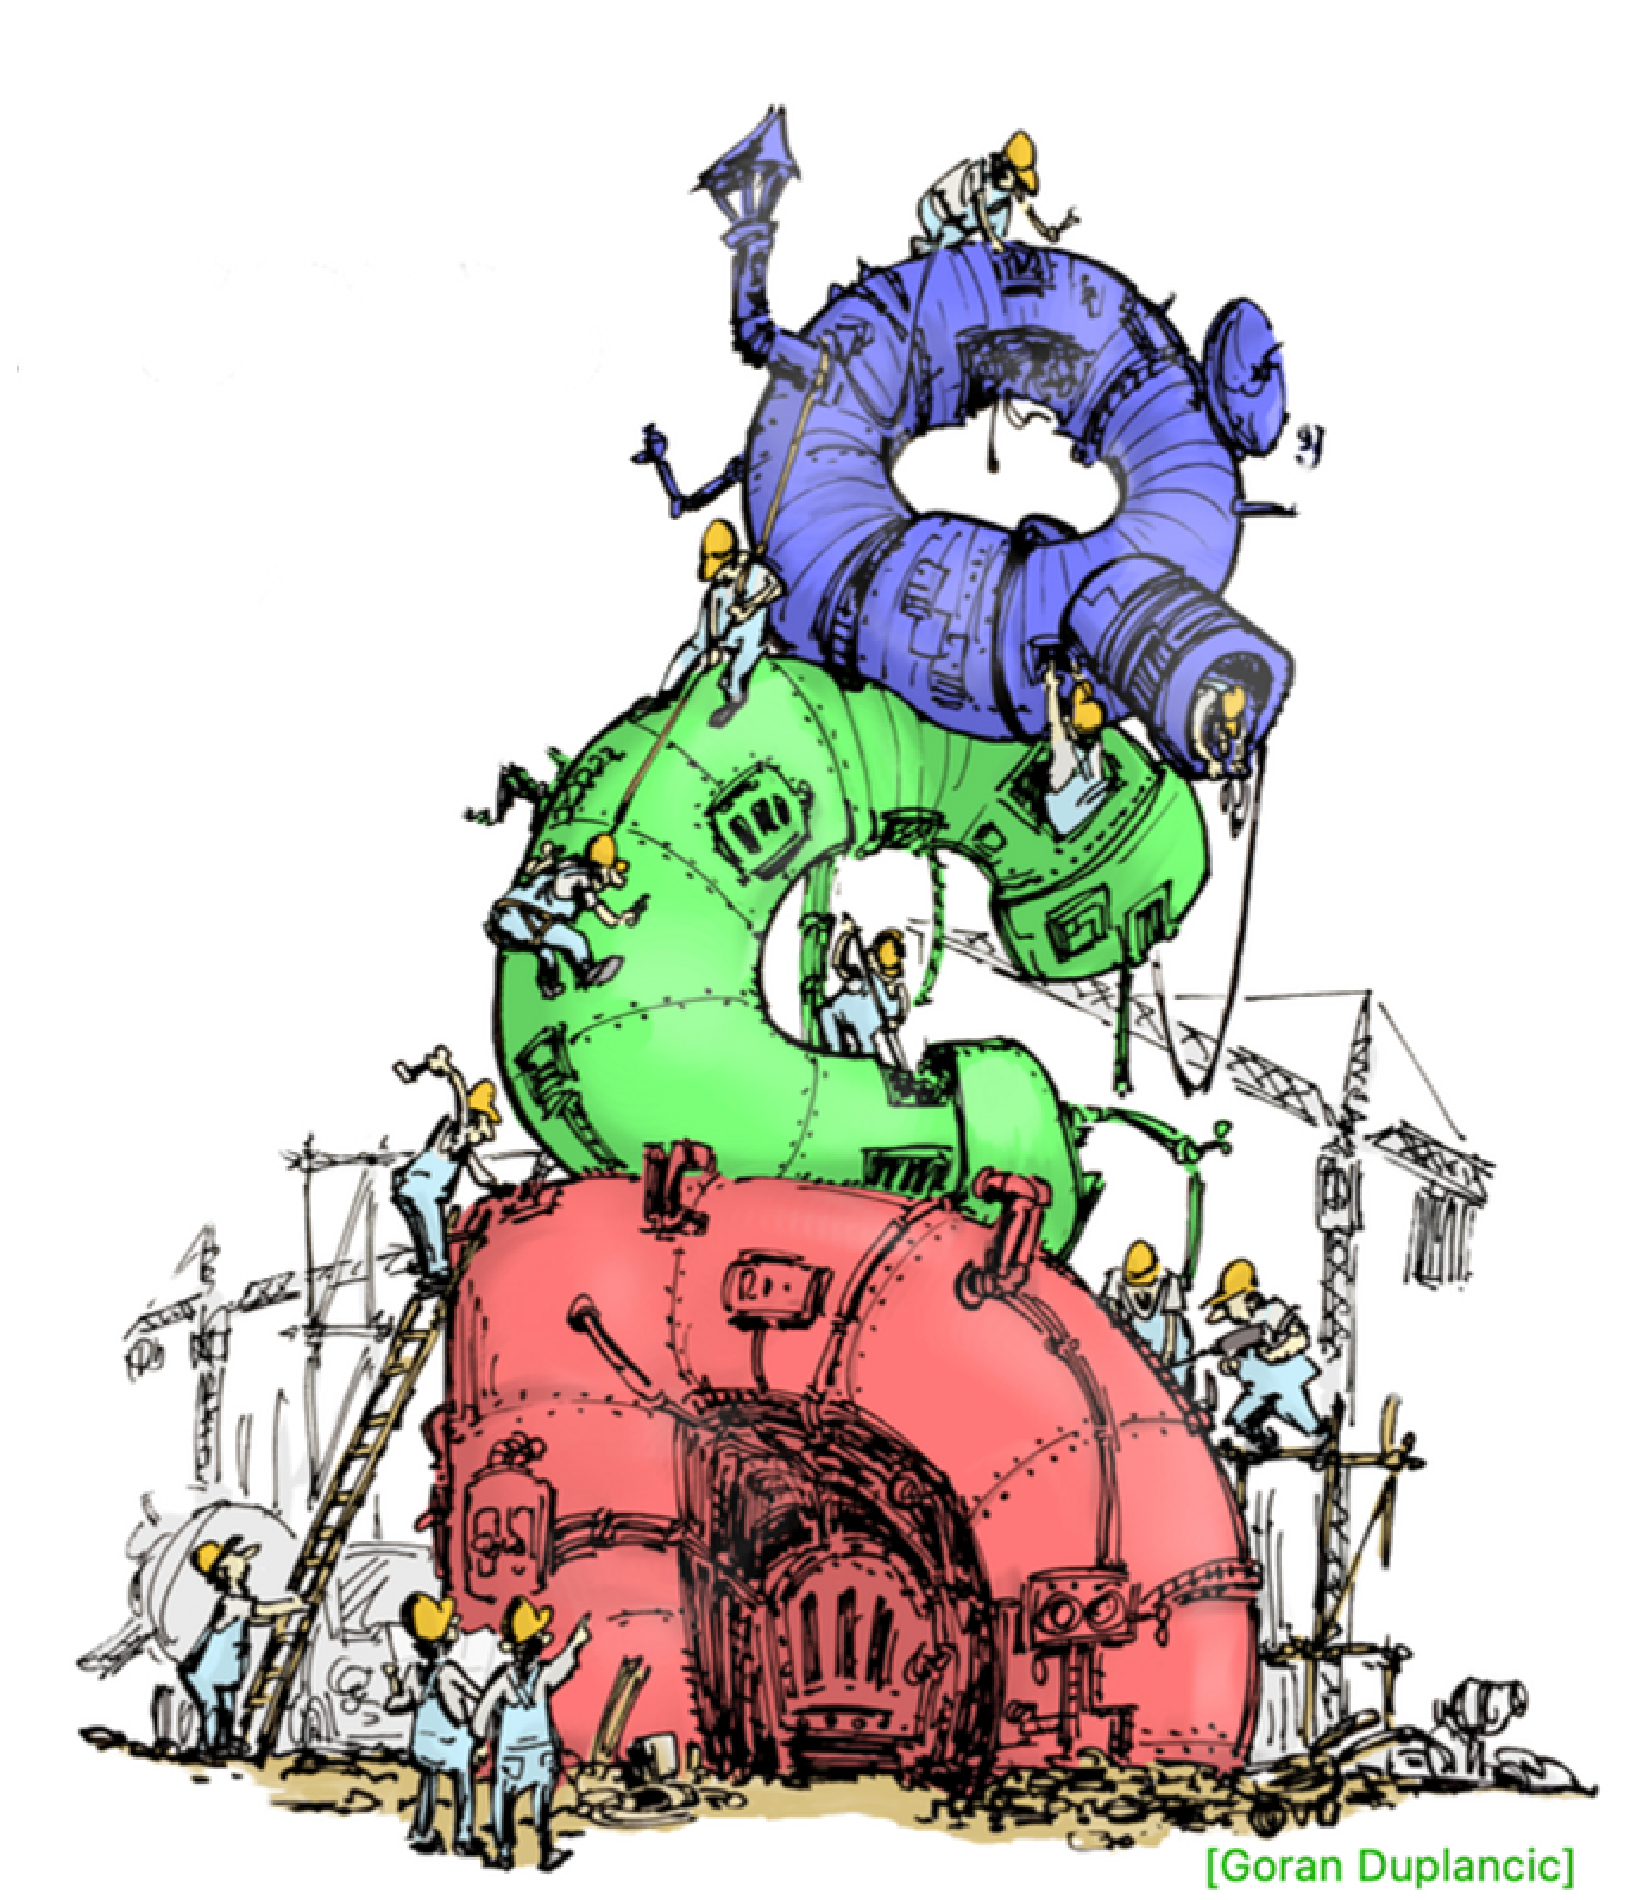
\includegraphics[scale=0.25]{sections/Chapters/Chapter1/Images/qcd.pdf}
    \caption{QCD is a colorful theory. A sketch by Goran Duplancic.}
\end{figure}

The QCD lagrangian is invariant under SU(3) color symmetry.

\begin{equation}
    \mathcal{L}_{QCD} = - \frac{1}{4} \sum_{a=1}^{8} F^a_{\mu \nu}F^{a \nu \mu} + \sum_{f=1}^{6} \overbar{\psi}_f^i
    (i \gamma^{\mu} (D_{\mu})_{ij} - m_f \delta_{ij}) \psi_f^j
\end{equation}


Let's discuss the indeces: $\mu$, $\nu$ are the usual Lorentz's indeces, $a$ is the gluon index, $f$ is the
flavour index, $i$ and $j$ are color indeces ($i$, $j = 1, 2, 3$).
Furthermore the lagrangian contains the Faraday's tensor and the covariant derivative:

\begin{align}
    &F^a_{\mu \nu} = \partial_{\nu} G^a_{\mu} - \partial_{\mu} G^a_{\nu} + g f^{abc}G_{\mu}^{b}G^c_{\nu} \\
    &(D_{\mu})_{ij} = \partial_{\mu} \delta_{ij} - i g \tau^a_{ij} G^a_{\mu}
\end{align}

where $f^{abc}$ are the structure's constant of the SU(3) group, $G^a_{\mu}$ is the gluon four-vector, 
$\tau^a$ are the SU(3) generators.

The main difference between the Strong and EW sector is that the spontaneous symmetry breaking 
mechanism is not necessary to describe quarks' masses, because the lagrangian's mass term is invariant 
under SU(3) symmetry.

\begin{figure}[h]
    \centering
    \includegraphics[scale=0.8]{sections/chapters/Chapter1/Images/Feynman_H_VV.pdf}
    \caption{Vertices of the SM. Top row: fermion-vector boson (Z, W, $\gamma$) interaction, gluon splitting, 
    (only for quarks), Yukawa coupling between Higgs and fermions.
    Middle row: Higgs couplings with two vector bosons and then a triple and 
    quadruple Higgs coupling. 
    Bottom row: triple and quadruple vector boson coupling and a HHVV coupling.}
\end{figure}


\begin{comment}

\subsection{Parton Model}


\subsection{Jets}

When studying high-energy collisions one often has to consider processes with gluons and quarks in the final state.
Quarks and gluons can be produced in numerous processes such as the decay of W, Z and H bosons.
However, these high-energy quarks and gluons are not directly observed in the final state of the collision.
They tend to undergo successive branchings at small angles, producing a series of collimated quarks and gluons. 
This cloud of collimated particle is often referred to as “parton shower".
The fact that this parton shower is collimated traces back to the collinear divergence of QCD.
Starting from a parton with high virtuality (of the order of the hard scale of the process), 
the parton shower will produce branchings into further partons of decreasing virtuality, 
until one reaches a non-perturbative (hadronisation) scale, typically of order $\Lambda_{QCD}$ ($\sim$ 1 GeV).
At this stage, due to confinement, these quarks and gluons will form hadrons.
Conceptually jets are collimated flows of hadrons.

\subsection{Jet algorithms}

After discussing the meaning and origin of jets in the introduction, we require an infrared-safe definition of 
jets. Historically, the first definition of a process with two jets was given by Sterman and Weinberg. 
They defined a process with two jets as a process in which it is possible to identify two cones of angle $\delta$, 
within which all the energy of the process is contained, with a discrepancy of at most $\epsilon$.
The Sterman-Weinberg's cross section has two equivalent definitions:

\begin{align}
    \sigma_{SW} &= \sigma^{q \bar{q}} + \sigma^{3 partons}(E_i < \epsilon \sqrt{s} \land \theta_{ij} < \delta) + \\
    + \sigma^{4 partons}(E_i < \epsilon \sqrt{s} \land \theta_{ij} < \delta) + ... \\
    &= \sigma^{tot} - \int_{R} \frac{\sigma^{tot}}{d x_1 d x_2}
\end{align}


The first definition defines the SW cross section as the sum of the cross sections with an increasing number 
of partons in the partonic final state. The cross section with two partons does not require any constraints 
since it naturally produces two jets. The cross section with three partons, in order to have two jets in the 
final state, requires constraints on the third parton, which must not form a jet. Hence, it must be either 
inside one of the cones ($\theta_{ij} < \delta$) or have an energy below the tolerance of $\epsilon \sqrt{s}$. 
Similarly, the cross section with four partons has the same constraints but on two partons instead of just one.

The second equivalent definition defines the SW cross section as the whole cross-section minus the hard 
cross-section.
The integration domain $R$ identifies the hard region of the Dalitz plot (i.e., the central one).


In the modern era the jet definitions are \textbf{jet algorithms} which are well-defined procedure that tells 
how to reconstruct the jets from the set of hadrons in the final state of the collision.
A jet algorithm has three main building blocks:

\begin{itemize}
    \item \textbf{Distance}.\\
    The distance expresses how much collinear or soft is an hadron.
    Therefore the definition of the distance plays a fundamental role to determine if an hadron lies within or
    outside a jet cone.
    The definition must be well-thought in order to avoid an unproper clustering procedure.
    \item \textbf{Cut}.\\
    The cut is the value that determines whether the hadron will be clustered to form a jet or not. 
    If it is too small, the algorithm would be too sensitive and would tend to identify a jet for each particle. 
    On the other hand, if it is too large, the algorithm tends to cluster every particle into a single jet.
    \item \textbf{Recombination Scheme}.\\
    The recombination scheme is the rule which builds the jet by recombining the four-momentum of particles
    that lie within the jet's cone.
    Examples of recombination schemes are the “E-scheme" and the “Winner Take All".
\end{itemize}

The workflow of a jet algorithm could be summarised by the flowchart shown in figure 
\end{comment}

\section{Quantum Computing in High Energy Physics}

The HEP and Quantum information communities have recently joined forces to investigate possible 
applications of Quantum Computing in High Energy Physics.
The recently published article by the QC4HEP Working Group \cite{dimeglio} summarizes these possible applications, which are divided in 
two main domain areas: theoretical methods and algorithms for modelling HEP problems, and numerical methods 
for the interpretation and analysis of experimental results (as well as detector simulation and event generation).\\
In the next two paragraphs I will briefly discuss this possible applications of QC to HEP.

\subsection{Quantum Computing for Theoretical Modelling in HEP}

Numerous theoretical simulations of lattice gauge theories rely on the widespread technique of euclidean 
path-integral Monte Carlo simulations.\\
However, this technique suffers from the \textit{sign problem}, which means that contributions 
to the path integral can cancel out, leading to numerical instability and increased computational cost.\\
Recently, Tensor Networks\footnote[1]{For an introduction on Tensor Networks \cite{Bridgeman_2017}.
For an introduction on the simulation of lattice gauge theories with Tensor Networks \cite{Dalmonte_2016}.} 
have become a popular alternative to circumvent the 
\textit{sign problem}.
Tensor Networks, which are based on the Hamiltonian formalism (as opposed to lattice gauge theory simulations 
that typically use the Lagrangian formalism), provide a powerful framework for efficiently parameterizing 
the \textit{physical corner} of a Hilbert space\footnote[2]{The physical corner of the Hilbert space is the 
subset that describes the low-energy states of a quantum system.}. 
This approach reduces the complexity of exploring the entire Hilbert space landscape by focusing on the 
relevant low-energy subspace.\\
A promising alternative to Tensor Networks are simulations on quantum computers, because the number of 
required qubit (the fundamental unit of information) grows linearly with the number of lattice sites.
In addition, by sharing with Tensor Networks the Hamiltonian formulation, quantum computations 
completely avoid the \textit{sign problem}.
Thus, quantum computers could be a potential framework to fully overcome the limitations 
outlined above for the simulation of lattice gauge theories and especially their real-time dynamics.


\subsection{Quantum Computing in HEP Experiments}

An experiment in HEP requires three different categories of algorithms:

\begin{enumerate}
    \item Detector operation.\\
    Detector operation algorithms allow detectors to efficiently obtain data that cleanly represents the 
    fundamental interactions of matter. Detectors like ATLAS and CMS feature very large amounts of very high 
    dimensional data, which requires algorithms that can handle such complex data.
    Moreover, these detectors require algorithms to sort significant signals from noise.
    \item Identification and reconstruction algorithms.\\
    Identification and reconstruction algorithms are an essential part of mapping the vast collection of 
    pixel intensities, timings, and event counts to a coherent underlying physics structure in the data.
    \item Simulation algorithms.\\
    Robust simulation and inference tools allow particle physics experiments to compare 
    large amounts of complex, highly structured data with parametrized theoretical predictions.
\end{enumerate}

Quantum Computing could play a fundamental role in each of the above-mentioned categories.\\
Experiments running on high-luminosity accelerators need faster algorithms and QC 
could be instrumental to speed-up the processing time of large datasets.
Moreover, quantum algorithms that leverage the unique properties of \textit{entanglement} and 
\textit{superposition} could potentially extract more information 
from a given dataset than classical algorithms.
Finally, quantum algorithms could capture more complex aspects of HEP theory and simulation providing 
estimators that are more natively aligned with the quantum mechanical nature of the Standard Model.

\begin{figure}
    \centering
    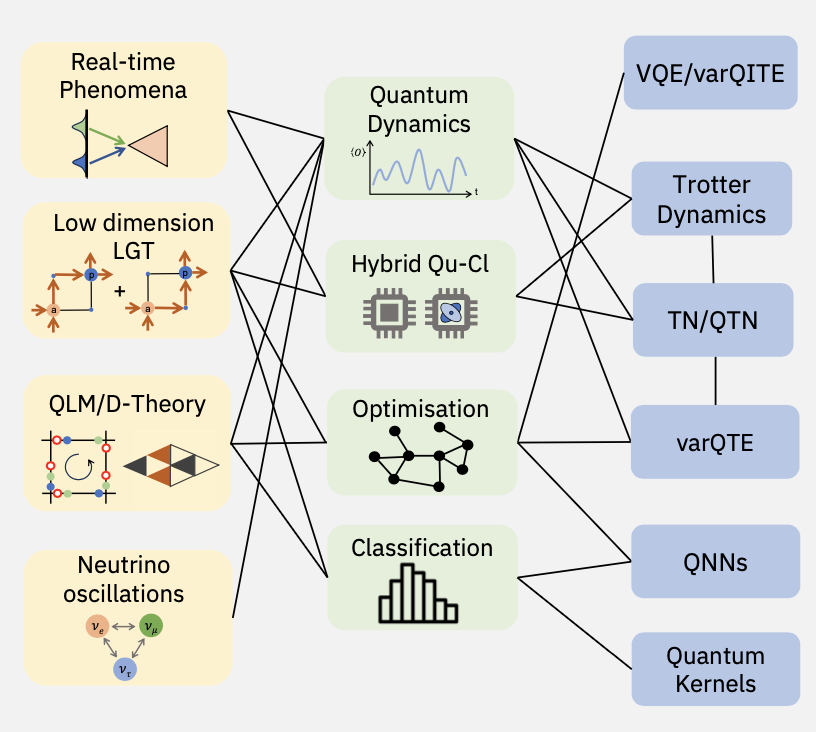
\includegraphics[scale=0.45]{sections/chapters/Chapter1/Images/exp-qc.png}
    \caption{In yellow, common High Energy Physics (HEP) tasks; in green, the corresponding machine 
    learning tasks; and in blue, the corresponding quantum algorithms.}
\end{figure}






    \clearpage
    
\chapter{Machine Learning}

The term \textit{Machine Learning} was coined in 1959 by Arthur Samuel, an IBM employee and pioneer in the field of computer gaming and 
artificial intelligence.
The term \textit{Machine Learning} is often interchanged with other terms, such as \textit{Deep Learning}, \textit{Artificial Intellingence} (AI) 
and \textit{Artificial Neural Networks} (ANN), but they have different meanings.\\
The correct hierarchy among these terms is illustrated in Figure~\ref{fig:venn-AI}, where it is evident that the broadest term is AI and it includes 
\textit{Machine Learning}, \textit{Deep Learning}, and \textit{Artificial Neural Networks}.
A possible definition of AI was given by John McCarthy, an American computer scientist regarded as one of the founders of the field: 
\textit{"AI is the science and engineering of making intelligent machines."} (1956).

\begin{figure}[h]
\centering
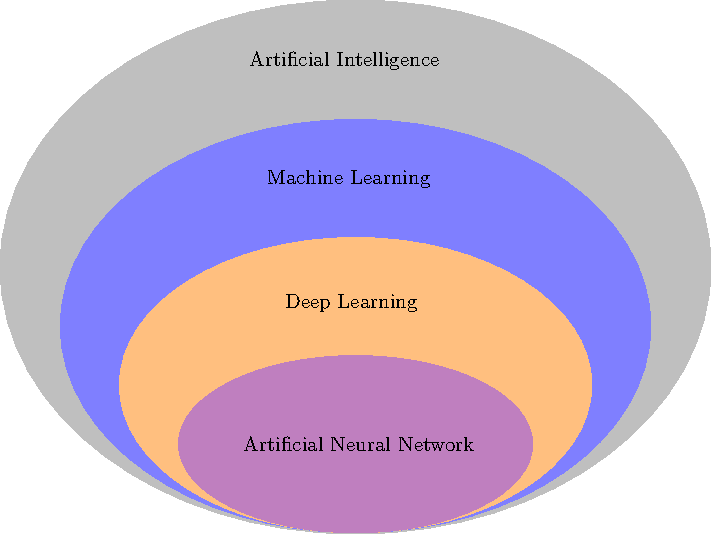
\includegraphics[scale=0.8]{Chapters/Chapter2/venn_diagram/venn.pdf}
\caption{Venn diagram representing the relationship between AI, Machine Learning, Deep Learning and ANN.}
\label{fig:venn-AI}
\end{figure}

The distinction between \textit{Machine Learning} and \textit{Deep Learning} is often overlooked, but the key difference lies 
in the complexity and depth of the architectures. \textit{Deep Learning} models feature deep, layered architectures, while \textit{Machine Learning}
models typically involve shallower architectures. Today, nearly every model with significant real-world applications is a \textit{Deep Learning} model.\\

The term \textit{Machine Learning} refers to more than 60 different algorithms and they can be divided in three main categories: 

\begin{enumerate}

\item \textbf{Supervised Learning}: the algorithm learns to map an input to an output,  based on example input-output pairs.
Two main tasks belong to this category: classification and regression;
\item \textbf{Unsupervised Learning}: the algorithm learns patterns from untagged data.
Two main tasks belong to this category: clustering, dimensionality reduction;
\item \textbf{Reinforcement Learning}: the algorithm learns from the actions of an agent in an environment.
Its main task is real-time decisions;

\end{enumerate}

The operative workflow of a \textit{Machine Learning} model could be summarized by a \textit{pipeline} of five modules:

\begin{enumerate}

\item Data collection and cleaning;
\item Choice of the model, the cost function and the optimizer;
\item Training of the model;
\item Cross-Validation of the model;
\item Optimisation;

\end{enumerate}

\begin{figure}[h]
\centering
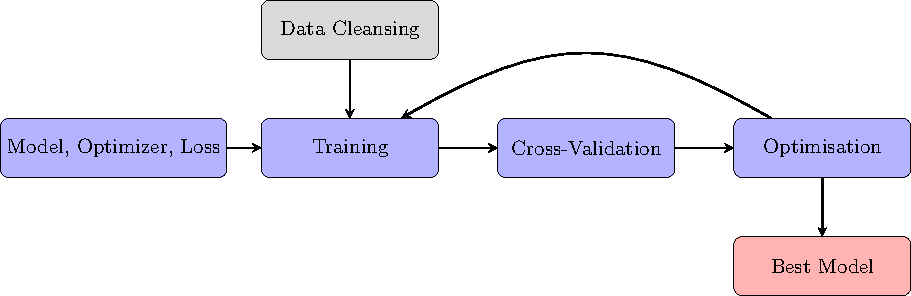
\includegraphics[scale=0.8]{Chapters/Chapter2/flowchart.pdf}
\caption{Pipeline of a machine learning algorithm.}
\label{fig:pipeline}
\end{figure}

I will provide a detailed explanation of these five steps within the context of supervised learning, which has been the central focus of my thesis.

\section{Supervised Learning}

Supervised learning is one of the three main categories of machine learning algorithms.
Its task is to infer a function of certain variables in order to predict other variables.

As shown in figure~\ref{fig:pipeline} the \textit{pipeline} specific to a supervised learning algorithm has different steps.\\

The first step is the \textit{collection}, \textit{evaluation} and \textit{cleaning} of the data.\\
It is essential to study, understand, clean and assemble the training data.
The term \textit{data cleaning} or \textit{data cleansing} refers to all kinds of tasks and activities to detect and repair errors in the data.\\

The second step is the \textit{choice} of the model, the metric and the optimizer.\\
This choice depends on the specific task.
For instance, two possible model choices for a classification task are: Artificial Neural Networks or Boosted Decision Trees.\\
Many different metrics exist and it is essential to choose the most appropriate for the specific problem.\\
The most popular optimisation algorithms are \textit{gradient-descent} based (Adam, Nadam, ...).
The basic idea underlying these algorithms is to find a minimum (local or global) of the loss function through an iterative process.
Therefore, the first step is to select a starting point, an initial vector $\vec{\omega}_0$, and then the algorithm keeps updating the vector of 
parameters $\vec{\omega}$ (or weights of the model) until it finds a minimun of the loss function.\\
Gradient-based optimisation algorithms update iteratively the weights of the model with this simple rule:

\begin{equation}
\omega_{t} := \omega_{t-1} - \alpha \frac{\partial}{\partial \omega_{t-1}} J(\vec{\omega}_{t-1})
\label{eq:update-param}
\end{equation}

where $\alpha$ is the \textit{learning rate} and t indicates the iteration.
The \textit{learning rate} is a tuning parameter which determines the step size at each iteration while moving toward a minimum of the loss function.
It represent the \textit{learning speed} of a machine learning model.
It is essential to carefully choose the learning rate, since, if $\alpha$ is too small gradient descent could be really slow, if $\alpha$ is 
too large gradient descent may fail to converge or diverge. \\
Gradient-based optimization algorithms (such as Adam, Nadam, Adamax, ...) differ from one another by introducing slight variations to the parameter 
update equation~\ref{eq:update-param}.
Among these, the most widely used is Adam (Adaptive Moment Estimation), which dynamically adjusts the learning rate for each parameter 
by estimating the first and second moments (mean and variance) of the gradients. The parameter update rule in Adam is given by:

\begin{equation}
    \omega_{t} := \omega_{t-1} - \alpha \frac{\hat{m_t}}{\sqrt{\hat{v_t}} + \epsilon} 
\end{equation}

where $\epsilon$ is a small constant added for numerical stability to prevent division by zero errors, whereas
The terms $\hat{m_t}$ and $\hat{v_t}$, as defined in the full Adam algorithm~\ref{work}, represent bias-corrected estimates of the first 
and second moments of the gradients:

\begin{align}
    \hat{m_t} = \frac{m_t}{1 - \beta_1^t}
    \qquad
    \hat{v_t} = \frac{v_t}{1 - \beta_2^t}
\end{align}

$m_t$ and $v_t$ are the exponentially weighted moving averages of the gradients and the squared gradients, respectively.
The hyperparameters $\beta_1$ and $\beta_2$ control the decay rates of these moving averages, with $\beta_1^t$ and $\beta_2^t$ representing 
these values at the timestep $t$.\\

\begin{algorithm}
    \caption{Adam, an algorithm for stochastic optimization. $g_t^2$ indicates the elementwise
    square $g_t \odot g_t$. Good default settings for machine learning problems are $\alpha = 0.001$,
    $\beta_1 = 0.9$, $\beta_2 = 0.999$ and $\epsilon = 10^{-8}$. All operations on vectors are element-wise. With $\beta_1^t$ and $\beta_2^t$
    I denote $\beta_1$ and $\beta_2$ to the power t.}
    \label{alg:adam}
    \begin{algorithmic}
    \Require $\alpha$: Stepsize
    \Require $\beta_1$, $\beta_2$ $\in [0, 1)$: Exponential decay rates for the moment estimates
    \Require $f(\omega)$: Stochastic objective function with parameters $\omega$
    \Require $\omega_0$: Initial parameter vector
    \State $m_0 \gets 0$ (Initialize $1^{st}$ moment vector)
    \State $v_0 \gets 0$ (Initialize $2^{nd}$ moment vector)
    \State $t \gets 0$ (Initialize timestep)
    \While{$\theta_t$ not converged}
    \State $t \gets t + 1$
    \State $g_t \gets \nabla_{\omega} f_t(\omega_{t-1}) $ (Get gradients w.r.t. stochastic objective at timestep t)
    \State $m_t \gets \beta_1 \cdot m_{t-1} + (1 - \beta_1) \cdot g_t$ (Update biased first moment estimate)
    \State $v_t \gets \beta_2 \cdot v_{t-1} + (1 - \beta_2) \cdot g_t^2$ (Update biased second raw moment estimate)
    \State $\hat{m_t} \gets m_t / (1 - \beta^t_1)$ (Compute bias-corrected first moment estimate)
    \State $\hat{v_t} \gets v_t / (1 - \beta^t_2)$ (Compute bias-corrected second raw moment estimate)
    \State $\omega_t \gets \omega_{t-1} - \alpha \cdot \hat{m_t} / (\sqrt{\hat{v_t}} + \epsilon)$ (Update parameters)
    \EndWhile
    \State \Return $\theta_t$ (Resulting parameters)
\end{algorithmic}
\label{work:adam}
\end{algorithm}

The third step is the \textit{training} of the chosen model.\\
In this stage the model is provided with observed data (x) and the label of the data (y), also known as \textit{target values}.
By providing to the model observed data (x) and the label of the observed data (y), the algorithm learns and adapts to map observed data to the labeled data.
For instance, in the training stage of an animal classifier algorithm, x would be images of animals and y the animal breed, hence the algorithm 
learns to connect the right label to a specific animal.\\

The fourth step is \textit{Cross-Validation}.\\
The input dataset is typically divided into two primary subsets: the \textit{training} set and the \textit{testing} set. 
The model will have an associated error for each of these subsets: one for the training dataset and another for the testing dataset.
However, in most cases, the dataset is further divided into three subsets: the \textit{training} set, the \textit{validation} set, and 
the \textit{testing} set. The inclusion of the \textit{validation} set addresses the issue of the \textit{bias–variance trade-off}.
The \textit{bias–variance trade off} is the conflict in trying to simultaneously minimize the bias error and the variance error.
Supposing we have model $\hat{y}(x)$ determined from a training data set, and considering as the true model:

\begin{equation}
    Y = y(x) + \epsilon
\end{equation}

where the noise $\epsilon$ has zero mean and constant variance.
Given a test set sample ($x_0$,$y_0$), the expected squared error can be expressed as:

\begin{equation}
    E[(y_0 - \hat{y}(x_0))^2] = (Bias[\hat{y}(x_0)])^2 + Var[\hat{y}(x_0)] + Var(\epsilon) 
\label{eq:variance-bias}
\end{equation}

where:

\begin{align}
Bias[\hat{y}(x0)] = E[\hat{y}(x_0)] - y(x_0)
\qquad
Var[\hat{y}(x_0)] = E[\hat{y}(x_0)^2] - (E[\hat{y}(x_0)])^2
\label{eq:variance-bias-errors}
\end{align}

Here, $Bias[\hat{y}(x0)]$ represents the bias of the model's prediction $\hat{y}(x_0)$ relative to the true value $y_0$, while 
$Var[\hat{y}(x_0)]$ indicates the variance of the model's predictions. The term $Var(\epsilon)$ represents the variance of the noise in the data.\\
Our objective is to minimize the expected squared error as described in equation~\ref{eq}.\\
High bias typically results in \textit{underfitting}, where the model fails to capture important relationships between the 
features and the target outputs, leading to poor performance on both training and test data. On the other hand, high 
variance results in \textit{overfitting}, where the model learns the noise in the training data rather than 
the underlying patterns, which impairs its performance on new, unseen data.
Therefore, the goal is to strike an optimal balance between bias and variance to avoid both underfitting and overfitting. 
This involves selecting a model that captures the true underlying patterns in the data without being too sensitive to fluctuations 
in the training data.\\
In order to reduce the \textit{bias–variance trade off} it is common to use cross-validation techniques, 
which divide the dataset in three groups: \textit{training} set, \textit{validation} set and \textit{testing} set.

\begin{figure}[h]
\centering
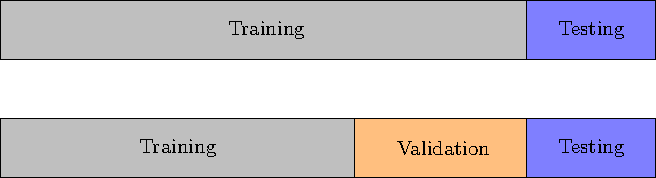
\includegraphics[scale=0.8]{Chapters/Chapter2/cross.pdf}
\caption{Comparison between the division of the data in two sets and three sets.}
\end{figure}

An example of a cross-validation technique is \textit{k-fold}.\\
This technique consists in splitting the training dataset in N folds (groups), where N-1 sets are unified and become the new \textit{training} set 
and the last one becomes the \textit{validation} set.
In rotation every single k-fold will be used as the \textit{validation} set once.\\

\begin{figure}[h]
\centering
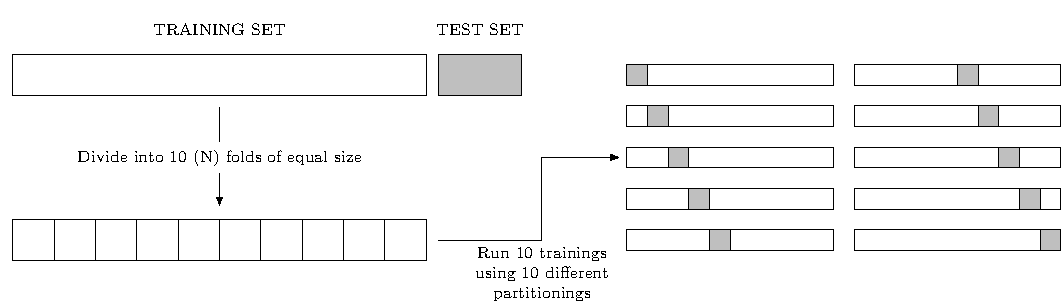
\includegraphics[scale=0.7]{Chapters/Chapter2/kfold.pdf}
\caption{Schematic explanation of the k-fold cross validation technique with 10 folds.}
\end{figure}


Finally, the fifth and last step is \textit{Optimization}. This step involves exploring the space of \textit{hyperparameters} to find the best 
configuration for the model. It typically includes adjusting parameters such as learning rates, batch sizes, and regularization terms to improve 
model performance and ensure optimal results.\\
Some common techniques for hyperparameter optimization are:

\begin{enumerate}
    \item Grid Search.\\
    Grid search involves defining a set of possible values for each hyperparameter and then exhaustively searching through all 
    possible combinations of these values.
    The great advantage of this technique is that it is easy to implement.
    However it can be unfeasible, because exploring every possible combination could be too computationally expensive.

    \item Random Search.\\
    Random search involves sampling hyperparameter values randomly from predefined distributions. Unlike grid search, 
    it does not evaluate all possible combinations but rather selects a subset of random configurations.
    It is often more efficient than grid search because it can explore a larger and more diverse set of combinations with fewer evaluations.
    The main disadvantage is that there is no guarantee that the best configuration will be found, as it only samples a subset of the 
    possible combinations.

    \item Genetic Algorithm.\\
    Genetic algorithms are inspired by the process of natural selection. They evolve a population of hyperparameter configurations 
    over multiple generations, using operations like mutation, crossover, and selection to find the best configurations.
    The main disadvantages are that it can be computationally expensive and it requires the tuning of internal parameters.

    \item Bayesian optimization.\\
    Bayesian optimization uses a probabilistic model to predict the performance of different hyperparameter configurations. 
    It iteratively selects the most promising configurations to evaluate based on past results, aiming to find the optimal set more efficiently.
    It can be more efficient than Grid Search and Random Search, but it requires a careful choice of the probabilistic model.

\end{enumerate}

In conclusion, the third, fourth and fifth steps can be repeated until the \textit{Best Model} is found.


\section{Artificial Neural Networks}

\textit{Artificial neural networks} (ANNs) are computing systems inspired by the biological neural networks that constitute animal brains.\\
An ANN can be visualised as \textit{layers} of \textit{neurons} (or \textit{node}), each of which receives inputs from all neurons in the previous layer.
A neural network has an \textit{input} and an \textit{output} layer and the layers in between are referred to as \textit{hidden}.
When the number of hidden layers (the network \textit{depth}) goes beyond one, the network is normally referred to as \textit{deep neural network} (DNN). 
The number of neurons in a given layer is referred to as its \textit{width}.

\begin{figure}[h]
\centering
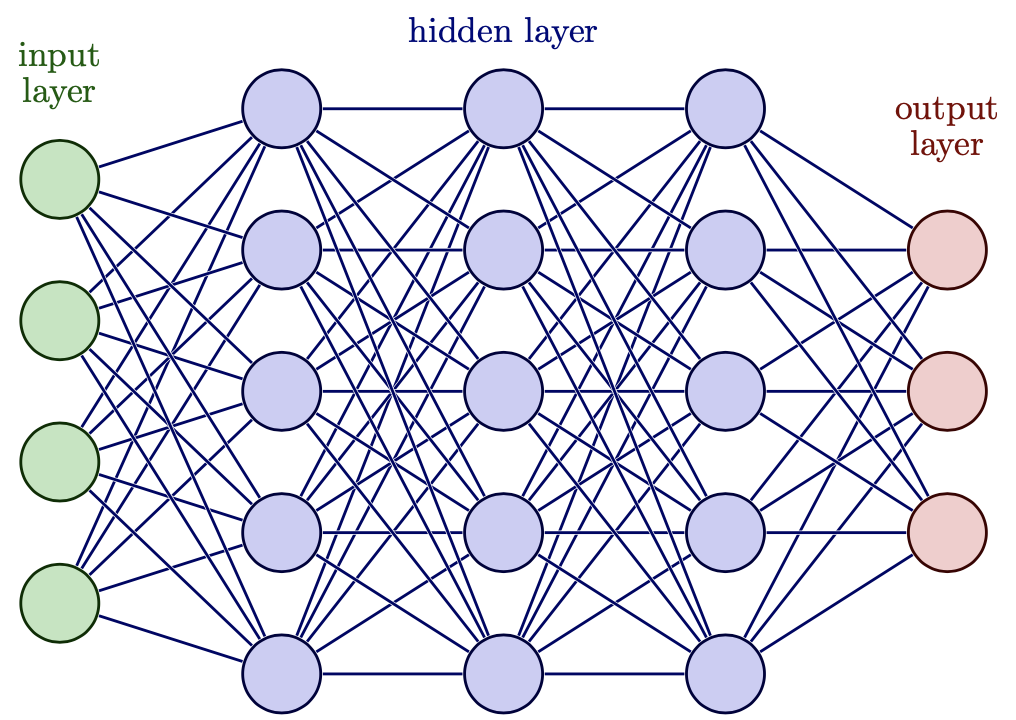
\includegraphics[scale=0.5]{Chapters/Chapter2/foto.png}
\caption{Multilayer perceptron with three hidden layers.}
\end{figure}

The neuron (or perceptron) is the fundamental unit of every ANN.
Each node combines linearly the input with \textit{weights} and a \textit{bias} and then its output is modulated by an \textit{activation function}, which introduces the non-linearity in the model.
Therefore the output of a node would be:

\begin{equation}
a = g(w_{0} + w_{1} x_1 + w_{2} x_2 + w_{3} x_3)
\end{equation}

where g is the activation function, $w_{0}$ is the bias and $w_{i}$ ($i \ne 0$) are the weights.

\begin{figure}[h]
\centering
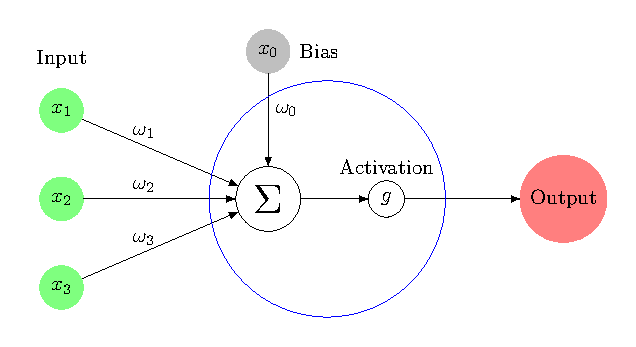
\includegraphics[scale=1]{Chapters/Chapter2/neuron.pdf}
\caption{Schematic representation of a neuron.}
\end{figure}


Many different activation functions exist: \textit{tanh}, \textit{sigmoid}, \textit{ReLU}, \textit{ELU}, ...\\
The training of an ANN is usually performed with gradient descent methods.
Since the number of weights could be copious, it is essential to use an algorithm which reduces the large amount of computations.
The \textit{backpropagation algorithm} is the most common algorithm to compute the gradient, since it can be used with any gradient-based optimizer.\\

There is a wide range of artificial neural network (ANN) architectures, ranging from simple models like the single perceptron to more complex ones 
such as Generative Adversarial Networks (GANs). Figure~\ref{fig:zoo} provides a partial overview of the diverse spectrum of neural network architectures.

\begin{figure}[h]
\centering
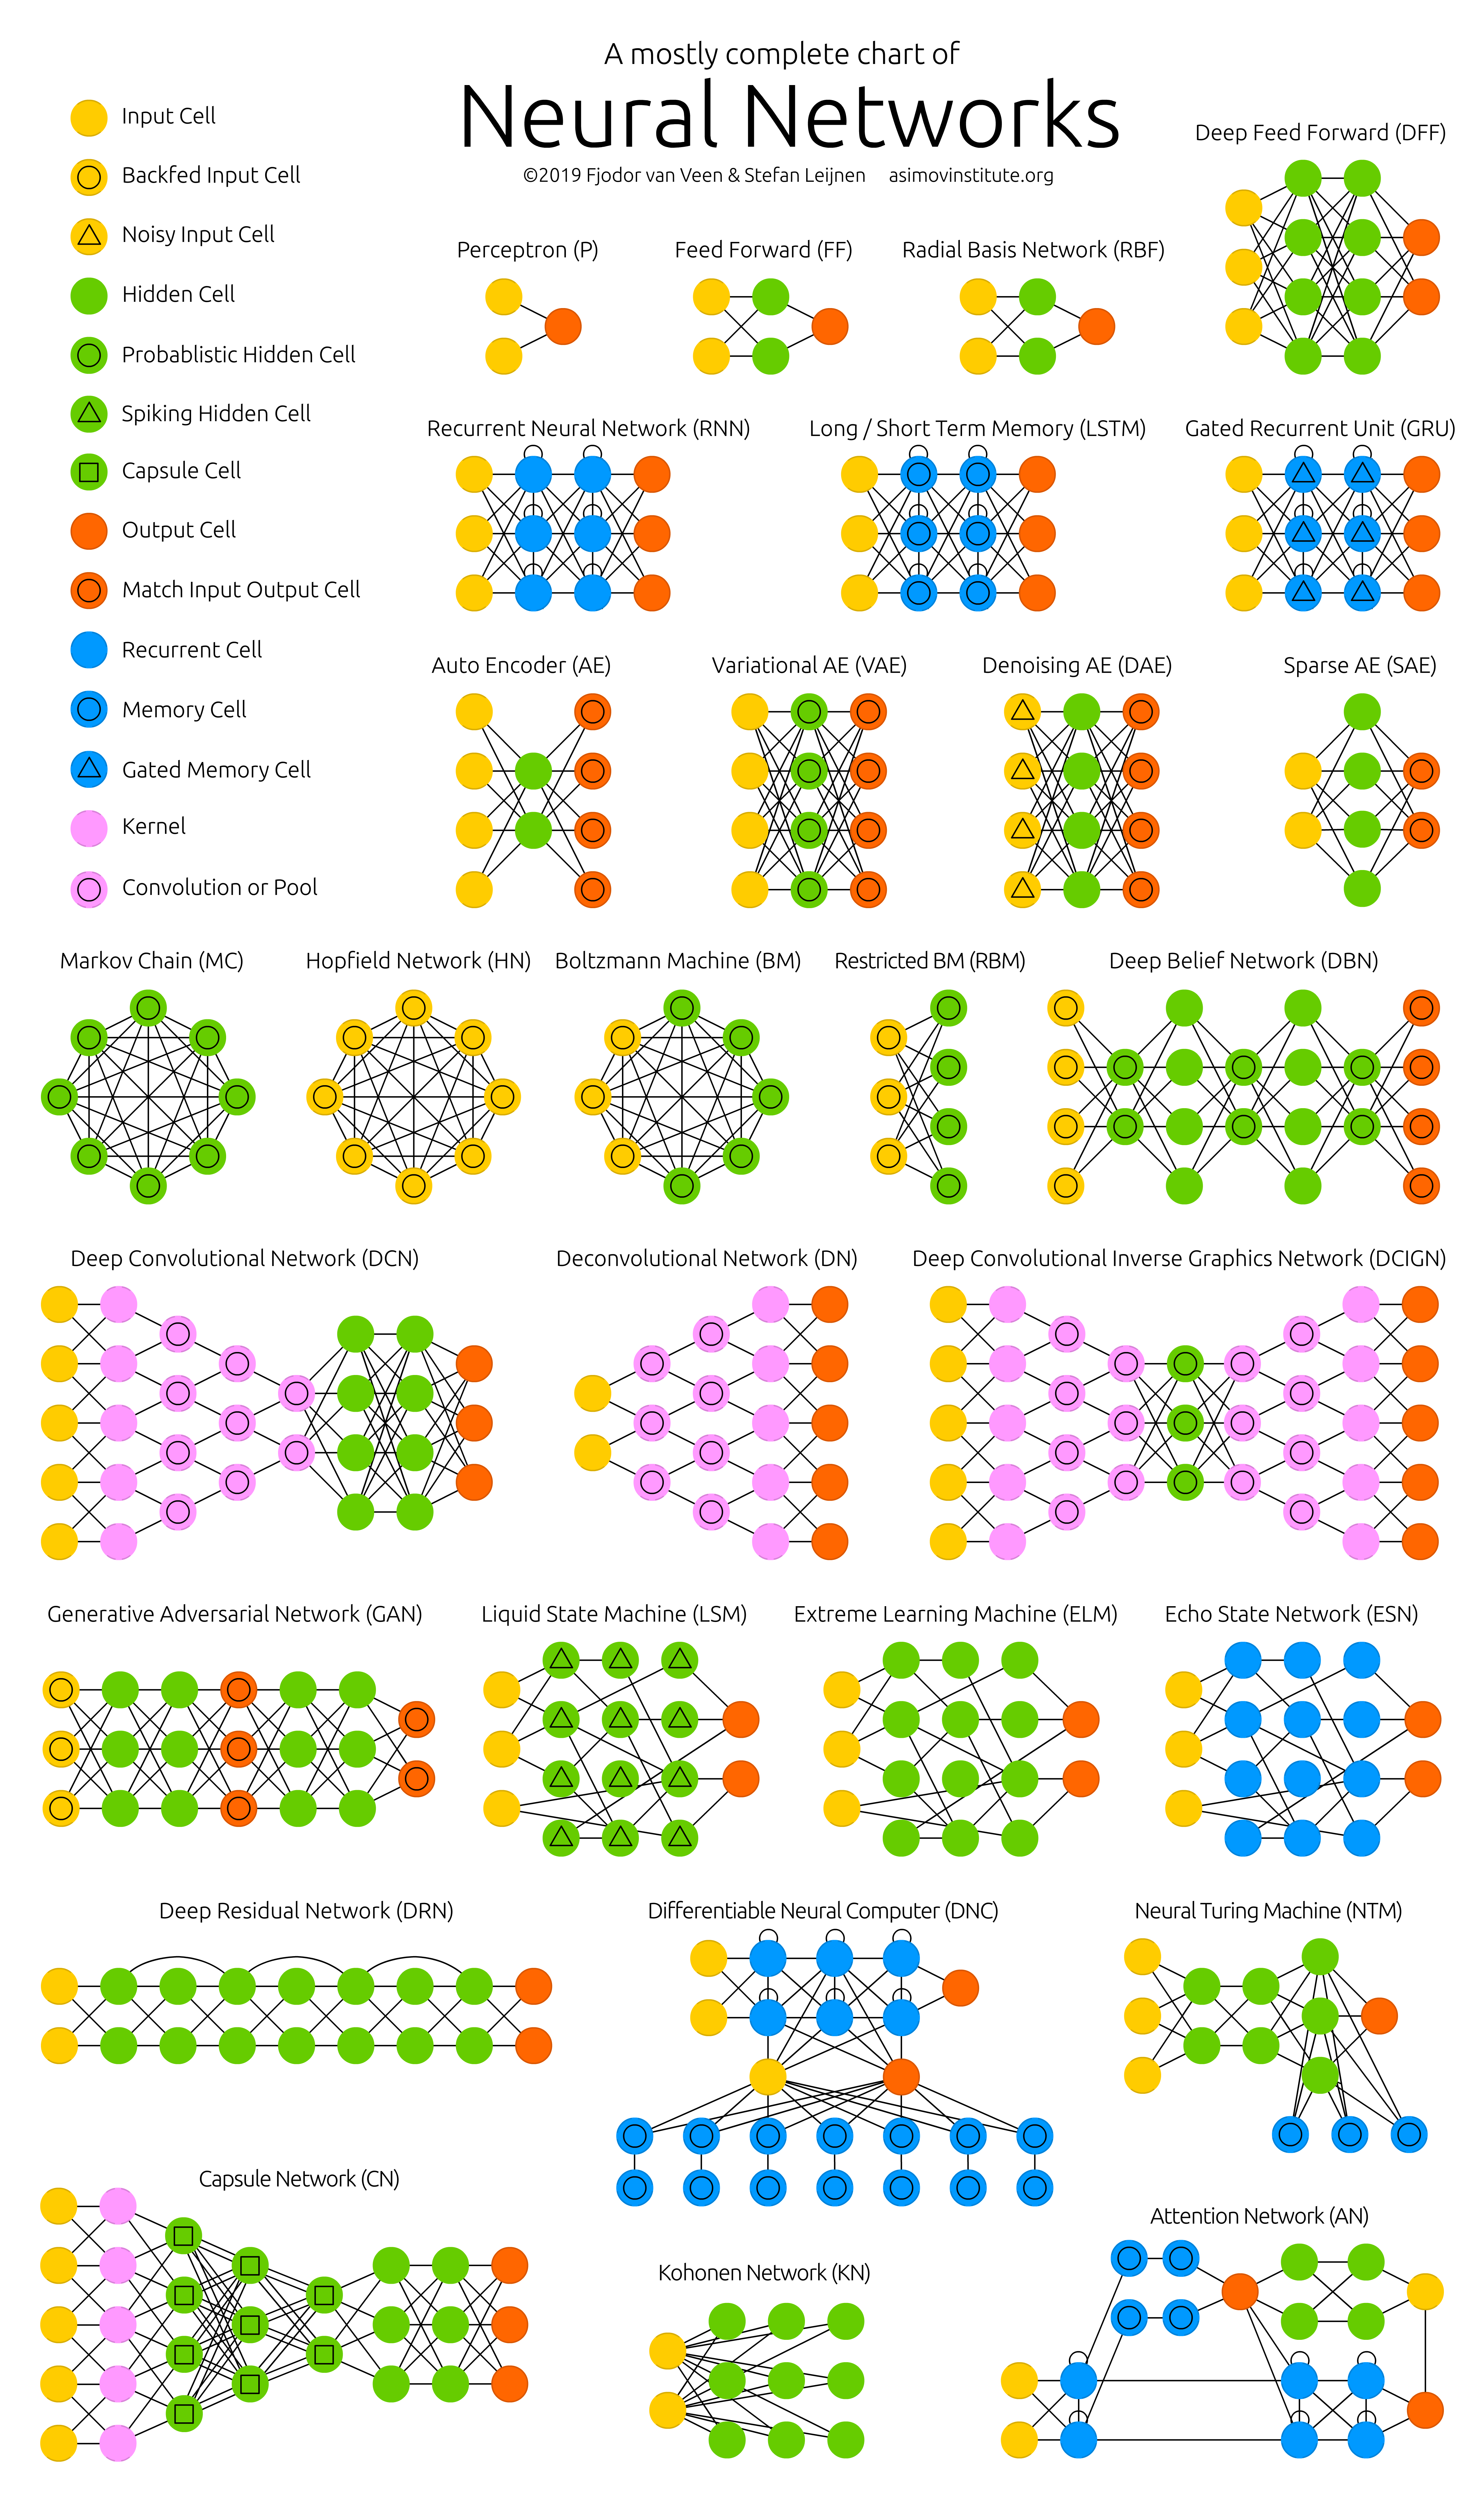
\includegraphics[scale=0.05]{Chapters/Chapter2/NeuralNetworkZoo.png}
\caption{Neural Networks Zoo.}
\label{fig:zoo}
\end{figure}

\subsection{Multilayer Perceptron}

A Multilayer Perceptron (MLP) is the builiding block of many ANN architectures.\\
It is a \textit{fully-connected} and \textit{feed-forward} artificial neural network.
The term \textit{fully-connected} means that each node of a layer is connected with every node of the previous layer.
The term \textit{feed-forward} means that connections between nodes do not form a cycle or a loop, hence the information moves in only 
one direction (forward) from the input nodes, through the hidden nodes and to the output nodes.


\subsection{Convolutional Neural Network}

Convolutional Neural Networks (CNNs) are a class of deep neural networks specifically designed to process and analyze grid-like data structures, 
such as images. CNNs are the standard architecture for tasks such as image 
classification, object detection, and image generation.\\

A CNN has two main components:

\begin{itemize}
    \item Convolutional Layer.\\
    Convolutional layers perform a convolution operation using filters (or kernels).
    Each kernel is a matrix of learnable weights that are updated during training.
    Each filter slides over the image with a certain stride (step size). At each position, 
    an element-wise multiplication (equation~\ref{eq:filter}) is performed between the filter and the portion of the input data it covers:

    \begin{equation}
        (I * K)(i,j)= \sum_m \sum_n I(i+m,j+n) \cdot K(m,n)
    \label{eq:filter}
    \end{equation}

    where (i,j) represents the position in the output feature map, and (m,n) indexes the filter matrix.
    This process enables the network to detect spatial hierarchies and essential features from the data.

    \begin{figure}[h]
    \centering
    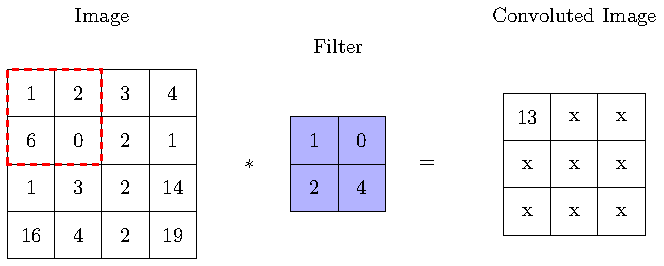
\includegraphics[scale=0.7]{Chapters/Chapter2/convolution/convolution.pdf}
    \caption{Convolution operation.}
    \end{figure}

    \item Pooling Layer.\\
    Pooling layers reduce the spatial dimensions of the feature maps while preserving important information. Common pooling techniques, 
    like max pooling and average pooling, help in minimizing computational complexity and making the network less sensitive to small translations 
    and distortions in the input data.

    \begin{figure}[h]
    \centering
    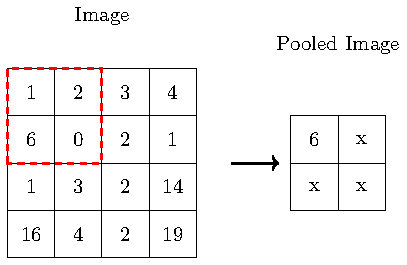
\includegraphics[scale=0.7]{Chapters/Chapter2/pooling/pooling.pdf}
    \caption{Max pooling operation.}
    \end{figure}
\end{itemize}

Following several convolutional and pooling layers, the high-level features are flattened and passed through a multilayer perceptron, which is
responsible for making final predictions based on the learned features.


\subsection{Binary and Multi-Class Classification}

Classification problems are supervised learning tasks for predicting variables that consist of a finite number of categories called
\textit{classes}. 
When the number of classes is two the classification problem is called \textit{binary-classification}, when the number of classes is larger than
two, the classification problems are called \textit{multi-class classification} problems. \\
Many different models could be used to deal with a classification task, such as K-Nearest Neighbors, Decision
Trees or Artificial Neural Networks.\\
The next two paragraphs describe the main features of binary and multi-class classifiers using as model an ANN.



\subsection{Binary Classifier}

A binary classifier distinguishes between two classes and therefore has a single node in the output layer. The output of this 
node is a probability score ranging from 0 (indicating the first class) to 1 (indicating the second class). To make a final 
classification decision, a \textit{discrimination threshold} must be set. This threshold determines the point at which the probability score is 
converted into a binary classification, effectively deciding which class the input belongs to based on the predicted probability.
A possible choice for the cost function of a binary classifier is the \textit{binary cross-entropy}:

\begin{equation}
J(\vec{\omega}) = - \frac{1}{n} \sum_{i=1}^n y_i log(\hat{y}_\omega(x_i)) + (1-y_i)(log(1-\hat{y}_\omega(x_i)))
\end{equation}

where $y_i$ is the target value, $\hat{y}_\omega(x_i)$ is the model output:

\begin{equation}
\hat{y}_{\omega}(x_i) = \frac{1}{1+e^{-\omega^Tx_i}}
\end{equation}

The output of a binary classifier can be visualized in a \textit{confusion matrix}.

\begin{figure}[h]
\centering
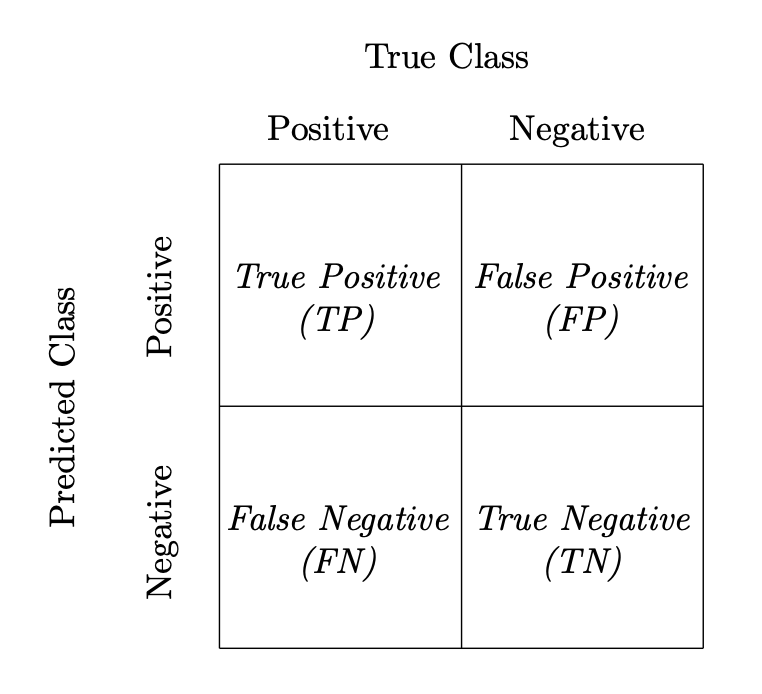
\includegraphics[scale=0.5]{Chapters/Chapter2/confusionmatrixdef.png}
\caption{Confusion matrix for a binary classifier.}
\end{figure}

Each row of the \textit{confusion matrix} represents the instances in a \textit{predicted class} while each column represents the instances 
in a \textit{true class} (or vicecersa).
In binary classification tasks the cost function is usually complemented with many other metrics based on the \textit{confusion matrix}:

\begin{itemize}

\item Accuracy:

\begin{equation}
Accuracy = \frac{TP + TN}{TP + TN + FP + FN}
\end{equation}

\item Precision:

\begin{equation}
Precision = \frac{TP}{TP + FP}
\end{equation}

\item Recall (or True positive rate):

\begin{equation}
Recall = \frac{TP}{TP + FN}
\end{equation}

\item False positive rate:

\begin{equation}
Recall = \frac{FP}{FP + TN}
\end{equation}

\item F1 score:

\begin{equation}
F1 = 2 \cdot \frac{Precision \cdot Recall}{Precision +  Recall}
\end{equation}

\end{itemize}

However these metrics depend on the discrimination threshold.
Therefore it is useful to introduce metrics which show the diagnostic ability of a binary classifier system as its discrimination threshold is varied:

\begin{itemize}

\item The \textit{ROC curve} plots the true positive rate against the false positive rate at various threshold settings;
\item The \textit{AUC} is the integral of the ROC curve;

\end{itemize}


\begin{figure}[h]
\centering
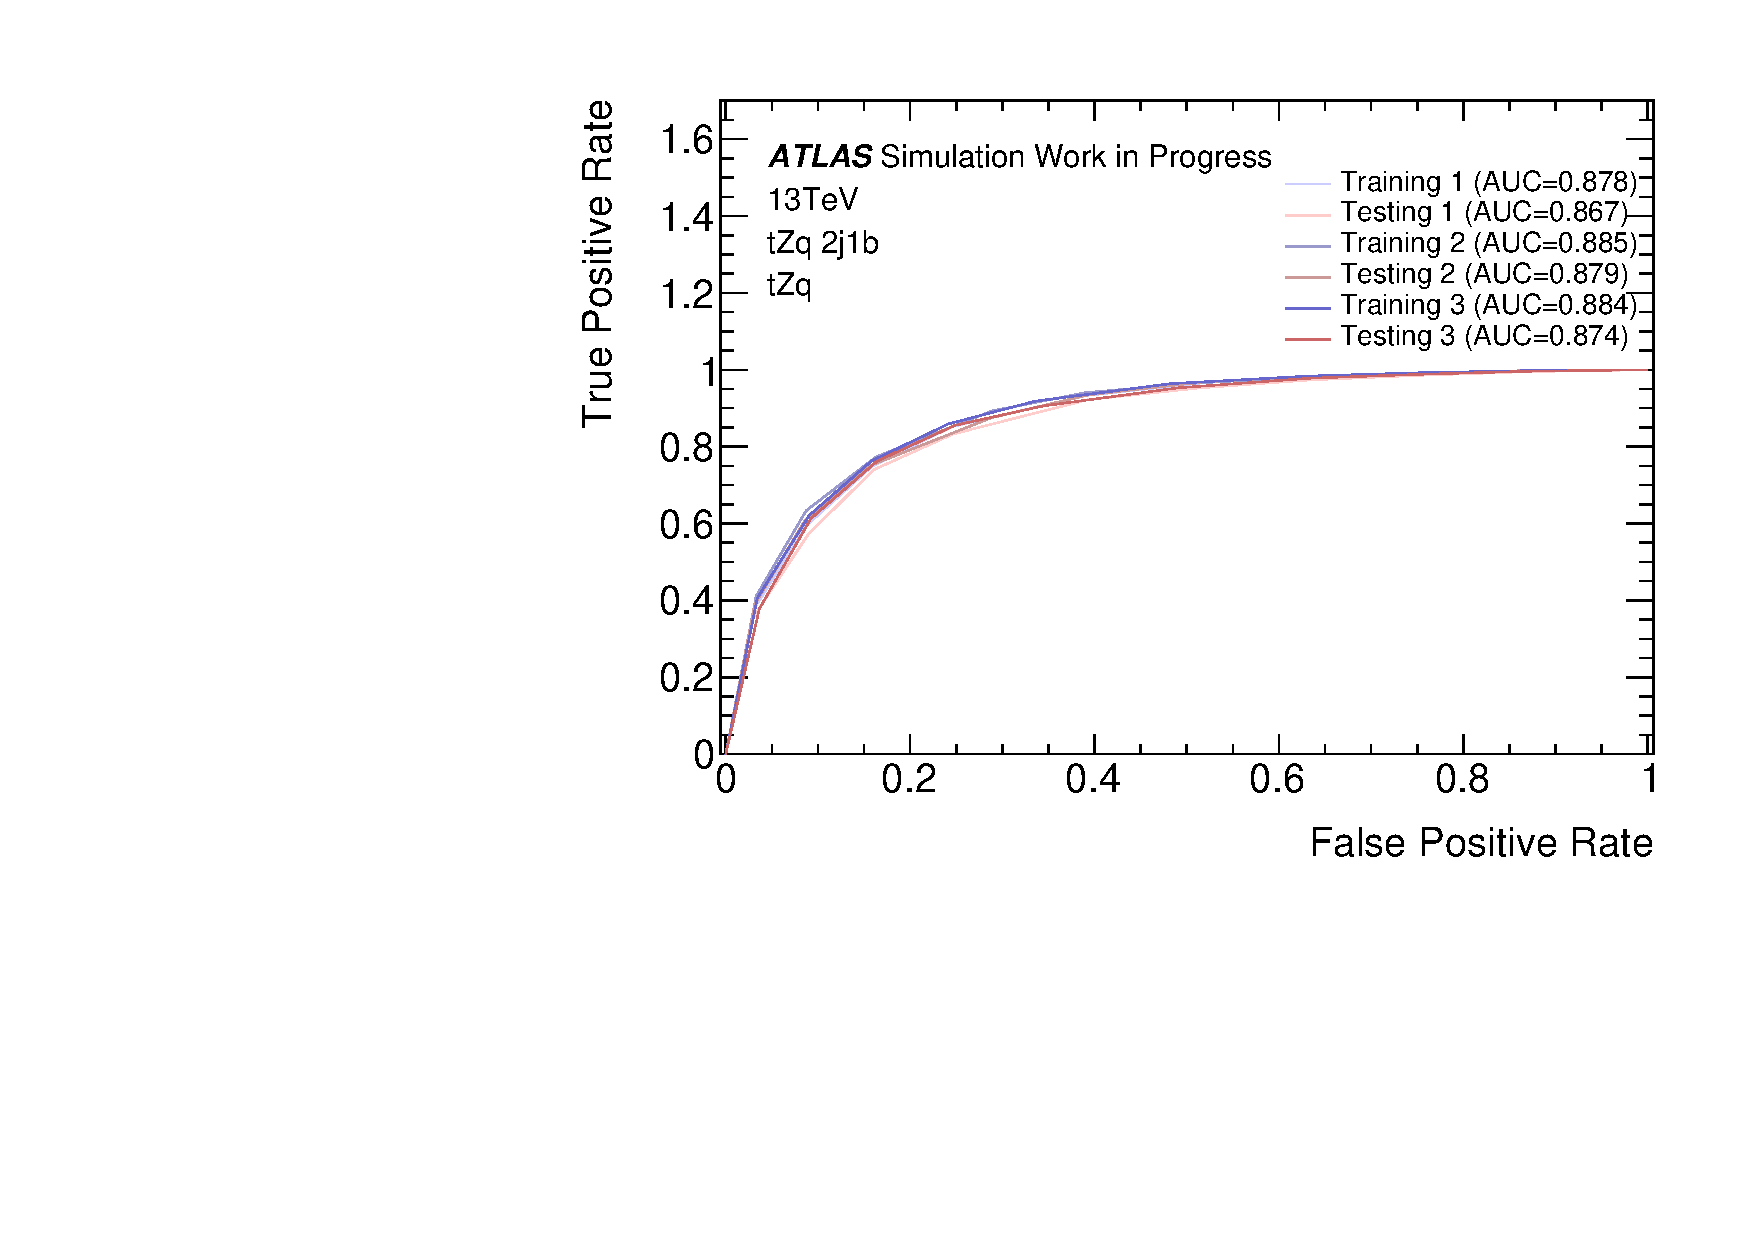
\includegraphics[scale=0.5]{Chapters/Chapter2/roccurve.pdf}
\caption{ROC curves for a three folded training of a binary classifier.}
\end{figure}

\subsection{Multi-class Classifier}
\label{section:multiclass_explanation}

There are two main strategies for solving a multi-class classification problem. 
The first is the use of classification algorithm which can solve the problem directly (K-Nearest Neighbors, Decision
Trees, Artificial Neural Networks). 
The second strategy is the decomposition of the original multi-class classification problem 
into several binary sub-problems (one-against-one or one-against-rest), and each sub-problem can be solved with a different 
classification algorithm.\\

A multi-class classifier has one node per class in the output layer.\\
Unlike a binary classifier whose output is modulated by a sigmoid, a multi-class network has as output a \textit{softmax} output. 
The \textit{softmax} function takes as input the vector of values of the output layer and converts them into probabilities associated to each class. 
Therefore the output of \textit{softmax} is a probability vector of three components for a multi-class classifier with three classes.

\begin{equation}
\sigma_i(\vec{x}) = \frac{exp(x_i)}{\sum^N_{i=1} exp(x_j)}
\end{equation}

The sum of the components of the \textit{softmax} output vector is normalized to one by definition.\\
The cost function of a multi-class classifier is the \textit{categorical cross-entropy}:

\begin{equation}
J(\vec{\omega}) = - \sum_{i=1}^{n} y_i log(\hat{y}_{\omega}(x_i))
\end{equation}


where $y_i$ is the i-th element of the vector $\vec{y}$ (the target vector) and represents the actual class, meanwhile $\hat{y}_{\omega}(x_i)$ represents the value of the i-th output.
The target vectors $\vec{y}$ for a three class classifier are three, one for each class:



\begin{align}
\vec{y}_1 = \begin{pmatrix}
1\\
0\\
0
\end{pmatrix}
\qquad
\vec{y}_2 = \begin{pmatrix}
0\\
1\\
0
\end{pmatrix}
\qquad
\vec{y}_3 =\begin{pmatrix}
0\\
0\\
1
\end{pmatrix}
\end{align}






    \clearpage
    \chapter{Quantum Machine Learning}

Quantum Machine Learning (QML) explores the interplay of ideas from quantum computing and
machine learning~\cite{Biamonte_2017}.
For example, QML investigates whether quantum computers can speed up the time it takes
to train or evaluate a machine learning model. On the other hand, the QML community
leverages techniques from machine learning to devise new quantum error-correcting codes~\cite{Roffe_2019}, 
estimate the properties of quantum systems, or develop new quantum algorithms.\\



The state of the art of Quantum Machine Learning has as main highlight the development
of algorithms that have been proven to have a quantum advantage in computational
complexity over classical algorithms~\cite{Sweke_2021, Liu_2021, Jerbi_2021}.
However, these algorithms require a fault-tolerant quantum computer~\cite{shor}, which is able to
continuously correct errors that arise during computation, ensuring the stability and
reliability of the quantum processes over extended periods.
As we are still many years away from fault tolerant quantum computation, the QML
community has developed a great interest toward possible applications of current and
near-term quantum devices (NISQ devices)~\cite{Preskill_2018}, which are not capable of continuous
quantum error correction.
In particular, the QML research community has developed a new class of quantum
procedures called variational quantum algorithms (VQA)~\cite{Cerezo_2021} to take advantage of current
and near-term quantum hardware.\\
However no quantum advantage has been proven for this algorithms, yet.\\

As previously stated, QML is the intersection of Machine Learning and Quantum Computing and this intersection can be 
factorised in four main areas:


\begin{itemize}
    \item \textbf{Classical for Classical (CC)}.\\ This area actually do not have a quantum component and 
    it indicates those purely classical cases when a classical machine learning algorithm is used to solve 
    a classical task.
    \item \textbf{Classical for Quantum (CQ)}.\\ This area indicates those studies which aim to use classical
    machine learning procedures to deal with problems in the quantum physics domain.
    \item \textbf{Quantum for Classical (QC)}.\\ This area instead refers to using quantum resources or algorithms, 
    for example variational quantum algorithms, to analyse or process classical information, 
    that is data that come from a classical source.
    \item \textbf{Quantum for Quantum (QQ)}.\\ This last area is arguably the most compelling yet unexplored
    application of Quantum Machine Learning, regarding the use of quantum processors to
    learn or study properties of quantum systems.
\end{itemize}

In my Master's thesis I have focused only on the \textit{Quantum for Classical} area.\\


In the next paragraphs I will briefly discuss Variational Quantum Algorithms, as they have been the focus
of my Master's thesis.


\section{Linear quantum models: explicit and implicit models}


\subsection{Explicit models}

A quantum machine learning model deals with data, thus the first step is to efficiently upload the data of the 
problem into the model.
Data can be either \textit{classical} $\{\bm{x}_i\}_{i=1}^m \in \chi \subseteq \mathbb{R}$ 
or \textit{quantum}, such as a set of states $\{ |\psi_i\rangle \}_{i=1}^m \in \mathcal{H} = C^{2n}$, 
where $\mathcal{H}$ is the Hilbert space of a quantum system of n qubits.\\
Let's discuss separately how to upload classical and quantum data on a quantum computer.

\begin{enumerate}
    \item Classical data.\\
    The procedure that uploads classical data $\{\bm{x}_i\}_{i=1}^m$ on a quantum computer is called
    \textit{feature embedding}.
    Specifically, this is achieved by a unitary $U(\bm{x})$ which depends on the data:

    \begin{align}
        \phi : \chi &\rightarrow \mathcal{F} = \mathcal{H}\\
        \bm{x} &\mapsto |\phi(\bm{x})\rangle = U(\bm{x}) |0\rangle^{\otimes n}\\
    \end{align}

    where $\mathcal{F}$ is the feature space, which in this case is the $\mathcal{H}$.
    We have numerous different feature embedding maps $U(\bm{x})$: \textit{angle encoding}, \textit{amplitude encoding},
    \textit{Qsample encoding}.\\
    For example the angle encoding consists in a different Pauli rotation for each component of the datapoint
    (thus requiring one qubit per dimension of the input data $d = n$):

    \begin{align}
        U(\bm{x}) = \otimes_{i=1}^n R_{P_i}(x_i) 
        \qquad 
        \bm{x} = (x_1, x_2, ..., x_N), P_i = {X, Y, Z}
    \end{align}

    In the amplitude encoding each component of a datapoint of dimension d becomes the amplitude of a vector 
    of the computational basis, thus requiring a number of qubit $n = \left\lceil log_2(d) \right\rceil$
    \footnote[1]{
        The amplitude encoding requires that the components of each datapoint $\bm{x}$ must be normalized. 
        This a fundamental restriction because 
        this means that quantum states represent the data one less dimension or with one less degree of freedom.
        For example a classical two dimensional vector $(x_1, x_2)$ can only be associated with an amplitude 
        vector $(\alpha_1, \alpha_2)$ of a qubit which fulfils $|\alpha_1|^2 + |\alpha_2|^2 = 1$.
    }.

    \begin{align}
    \bm{x} = \begin{pmatrix}
        x_1 \\
        x_2 \\
        ... \\
        x_{2^n} \\
    \end{pmatrix}
    \qquad
    \rightarrow
    \qquad
    \psi = \sum_i^{2^n} x_j | j \rangle
    \end{align}

    \item Quantum data.\\
    If we want to upload a certain quantum state $|\psi_i\rangle$ on a quantum computer, we have to determine
    the appropriate unitary $U_i$, which applied to the ground state gives $|\psi_i\rangle$:
    
    \begin{equation}
        U_i |0\rangle^{\otimes n} = |\psi_i\rangle
    \end{equation}
\end{enumerate}

Suppose we are given a classical dataset, thus we have to map these datapoints to an appropriate Hilbert space

\subsection{Implicit models}


\section{Variational Quantum Algorithms}

Variational Quantum Algorithms~\cite{Cerezo_2021} are the leading proposal to exploit current quantum computing platforms, 
based on the hope that it is possible to achieve a meaningful quantum advantage already in the non error-corrected 
regime, before standard quantum algorithms, like Shor’s factoring algorithm~\cite{Shor_1997}, can be realised at scale.\\ 

A VQA is a \textit{hybrid quantum-classical} algorithm with different components:

\begin{enumerate}
    \item \textbf{Encoding block}.\\
    The first component is the encoding block, which is responsible to encode the data of the problem in the 
    algorithm.
    \item \textbf{Parametrized Quantum Circuit (PQC)}.\\
    The second component is a parametrized quantum circuit U($\theta$), which is a circuit made of numerous gates. The parameters are usually 
    the angles of the circuit and they can be tuned to enhance the algorithm's performance for completing a specific task. 
    \item \textbf{Decoding Block}.\\
    The third component is the decoding block, which consists in measuring the PQC.
    \item \textbf{Optimization}.\\
    The valuable information extracted when measuring the PQC is used to evaluate a objective function.
    This objective function is then optimized, and this procedure suggests improved candidates 
    for the parameters $\theta$, starting from random or pre-trained initial values.
\end{enumerate}

The crucial point to emphasize of a VQA is that the PQC can be executed on current quantum
devices, while the computational demanding task of optimizing the objective function is
performed by a classical computer, which is far more reliable then current NISQ devices.
Therefore, the trademark of VQAs is that they use a quantum computer to estimate the cost function (or its gradient) 
while leveraging the power of classical optimizers to train the parameters: this is why they are called
\textit{hybrid quantum-classical} algorithms.\\
Many different VQAs have been designed to tackle standard machine learning tasks, such
as classification, regression or optimization.
CITAZIONE

\subsection{Parametrized Quantum Circuit}


Parameterized Quantum Circuits are the core of every VQA.\\
Consequently, it is crucial to design circuits that are not only \textit{easy to train} but also capable of 
\textit{generalizing} from the training data and sufficiently \textit{expressive} to identify an optimal solution 
for the given task.\\

A PQC, also known as \textit{quantum neural network}, can be expressed as a series of L parametrized unitaries:

\begin{equation}
    U(\theta) = \prod_{i=1}^L U_i(\theta_i)
\label{Eq:definition-PQC}
\end{equation}

where $\theta = (\theta_1, ..., \theta_L)$ is a set of tunable parameters.
This parameters are updated by optimizing a loss function:

\begin{comment}
\[
    \ell_{\theta}(\rho, O) = \text{Tr}\left[\rho(\theta)O\right]
    \qquad
    \rightarrow
    \qquad
    \argmin_{\theta} l_{\theta}(\rho, O)
\]
\end{comment}


More general loss functions exist, but this case is already relevant.\\
The main properties of a PQC are \textit{expressivity}~\cite{hubregtsen2020, Sim_2019, Bravo_Prieto_2020, 
Wu_2021, Herman_2023, Haug_2021, Holmes_2022}, \textit{generalization}~\cite{Caro_2020, Abbas_2021, Banchi_2021,
Bu_2023, bu2021, Bu_2022, Du_2022, Peters_2023, Caro_2023} and \textit{trainability}~\cite{McClean_2018, 
Cerezo_2021, Arrasmith_2021, Kim_2021, Wang_2021, Pesah_2021, marrero2021, Larocca_2023}.

\paragraph{Trainability}

As in classical machine learning, variational quantum algorithms can suffer from the problem of vanishing 
gradient, or in QML terms \textit{Barren Plateaus} (BP).
A common definition of BP for VQAs is the following:

\begin{defn*}[Barren Plateaus]
    A VQA exhibits a BP if its loss function, or its gradients, concentrate exponentially about their mean 
    in the number of qubits n
    \footnote[1]{The two definitions of Barren Plateaus — one involving gradients and the other 
    involving the loss function — are not equivalent. The definition based on the loss function is 
    unambiguous, whereas the definition in terms of partial derivatives can be less clear. The ambiguity 
    arises because some partial derivatives might be exponentially concentrated while others are not. In such 
    cases, the loss function would not exhibit exponential concentration, indicating that the two definitions 
    are not equivalent. They become equivalent only when \textit{all} the gradients are exponentially concentrated 
    \cite{Arrasmith_2022}.}.
\end{defn*}

This means that, as the number of qubits n increases, the gradients of the loss function (or the loss function itself) 
tend to concentrate around an average value with increasing probability.    
The average value around which the gradient must concentrate in order to exhibit BP must be very 
small\footnote[1]{\cite{McClean_2018} demonstrated that, under broad conditions, random parameterized quantum 
circuits have an average gradient value of zero.}.
In fact, if the gradient were concentrated around a non-infinitesimal value, it would mean that the 
algorithm is still learning.
Intuitively, this means that the optimization landscape is mostly flat and featureless and
that slightly changing the model’s parameters $\theta$ results in only an exponentially small change in the loss
function value or its gradient.\\

The probabilistic nature of Quantum Mechanics forces us to measured a finite amount of times N the PQC to determine
the average value of an observable.
The statistical uncertainty related to the average value is inversely proportional to $\sqrt{N}$.
Therefore, if the loss function has an exponential concentration (which means that the changes of the loss function 
from one epoch to the following are exponentially suppressed), we need an exponential amount of shots to resolve this
changes, rendering the algorithm inefficient and non-scalable.
 

Two main types of BPs exist:

\begin{comment}
\begin{enumerate}
    \item \textbf{Probabilistic concentration and narrow gorges}.\\
    The most common type of BP is known as \textit{probabilistic concentration}.

    \begin{equation}
        Var_{\theta} \[ \ell_{\theta}(\rho, O) \] or Var_{\theta} \[ \partial_{\mu} \ell_{\theta}(\rho, O) \] \in \mathcal{O}(\frac{1}{b^n})
    \end{equation}

    where $b > 1$. Chebyshev's inequality implies for any $\delta > 0$:

    \begin{align}
        Pr(|\ell_{\theta}(\rho, O) - \mathbb{E}_{\theta}(\ell_{\theta}(\rho, O))| \ge \delta) \in \mathcal{O}(\frac{1}{b^n})\\
        Pr(|\partial_{\mu} \ell_{\theta}(\rho, O) - \mathbb{E}_{\theta}(\partial_{\mu} \ell_{\theta}(\rho, O))| \ge \delta) \in \mathcal{O}(\frac{1}{b^n})\\
    \end{align}

    which means that the probability that the loss deviates from its mean is exponentially small.\\
    Probabilistic BP imply a mostly flat landscape with some \textit{narrow gorge}.
    
    \item \textbf{Deterministic concentration}.\\
    A deterministic BP arises when $\forall \theta$:
    \begin{align}
        |\ell_{\theta}(\rho, O) - \mathbb{E}_{\theta}(\ell_{\theta}(\rho, O))| \in \mathcal{O}(\frac{1}{b^n})\\
        |\partial_{\mu} \ell_{\theta}(\rho, O) - \mathbb{E}_{\theta}(\partial_{\mu} \ell_{\theta}(\rho, O))| \in \mathcal{O}(\frac{1}{b^n})\\
    \end{align}

    where $b > 1$.
    Deterministic BP do not even admit narrow gorges.
\end{enumerate}
\end{comment}

A possible method to determine if the loss or the gradients are concentrating was introduced by \cite{McClean_2018}.
They randomly sampled parameters and computed how the variance scales with the number of qubits 
(figure \ref{figure:McClean}).
In particular, this paper showed that for a large class of random quantum circuits the average value of the gradient of the objective 
function is zero and the probability that any given instance of such a random circuit deviates from this average 
value by a small constant $\epsilon$ is exponentially small in the number of qubits.
The region where the average value of the gradient is zero does not correspond to a local minimum, but rather an 
exponentially large plateau in the landscape of the parameters.\\

\begin{figure}
    \centering
    \includegraphics[width=.45\textwidth]{sections/chapters/Chapter4/Images/ProjectionGradientVar.pdf}
    \includegraphics[width=.45\textwidth]{sections/chapters/Chapter4/Images/ProjectionGradientVarLayers.pdf}
    \caption{These are the original images from the paper by \cite{McClean_2018}. 
    The image on the left shows the variance of the gradient of a two-local Pauli term plotted as a function of 
    the number of qubits: an exponential decay is observed as a function of the number 
    of qubits for both the expected value and its spread.
    The image on the right shows the variance of the gradient of a two-local Pauli term plotted as a function of the 
    number of layers. The different lines correspond to all even numbers of qubits between 
    2 and 24, with 2 qubits being the top line, and the rest being ordered by qubit number. This shows 
    the convergence of the variance as a function of the number of layers to a fixed value determined by the 
    number of qubits.
    }
    \label{figure:McClean}
\end{figure}

Other possible quantities have introduced to study if a BP occurs: \textit{landscape's information content} \cite{P_rez_Salinas_2024}, 
\textit{local state's entanglement} \cite{Sack_2022}, \textit{landscape's Fourier coefficients} \cite{okumura2023, Nemkov_2023}.

The final remark on trainability is to discuss the origin of BPs:

\begin{itemize}
    \item \textbf{Curse of dimensionality}.\\
    \item \textbf{Circuit expressiveness}.\\
    \item 
\end{itemize}

\paragraph{Generalization}


\paragraph{Expressivity}



\section{Quantum Machine Learning}

\subsection{Linear quantum models: quantum classifiers and kernel methods}

\subsection{Data reuploading models and Quantum Neural Network}

\subsection{Deriving the Fourier expansion}

\subsection{A single-qubit data reuploading circuit}

\subsection{Quantum Neural Networks}

\subsection{Generalization of QML models}

\subsection{The power of quantum machine learning}








    \clearpage
    
\chapter{A novel data encoding technique}

The paper \cite{P_rez_Salinas_2020} is a groundbreaking paper in quantum machine learning.\\
Significant effort by the quantum machine learning community has been dedicated to deepening our understanding of 
quantum re-uploading models, leading to a growing body of literature investigating them.\\
As we studied this paper, some natural questions emerged and we decided to investigate them by designing
a novel data encoding technique for quantum re-uploading models, whose main goal is to classify 
\textit{high-dimensional} and \textit{structured} datasets\footnote[1]{The term \textit{structured} is 
used to indicate that the components of each datapoint in the dataset may be highly correlated.}.\\
In the following sections we will discuss the questions emerged from reading the original data re-uploading
paper and a new quantum machine learning algorithm.

\section{Questions on data re-uploading}

The groundbreaking paper on the data re-uploading technique \cite{P_rez_Salinas_2020} does not address some crucial 
question, which could be an interesting starting point for future research:

\begin{itemize}
    \item\label{question:first} Is this encoding technique effective when dealing with high-dimensional datasets?\\
    The investigation conducted by Salinas et al focused on 2D, 3D and 4D data, hence this raises the natural
    question if this encoding method can deal with datasets of higher dimension.
    \item\label{question:second} Is this encoding technique effective when dealing with structured dataset (as images)?\\
    The original paper tested the data re-uploading encoding method to distinguish if a certain point was 
    inside or outside a certain geometrical boundary (circle, sphere, annulus, ...).
    However it did not investigate its performance on datasets, whose each datapoint's components could 
    be correlated to each other.
    Therefore, this raises another natural question which is if the data re-uplaoding technique can handle datasets
    like images, whose pixels are highly correlated to the sorrounding pixels.
\end{itemize}

We tried to answer to these questions by designing a new quantum machine learning algorithm based on the
data re-uploading technique.\\
I will discuss this new algorithm in the following section.

\section{Block re-uploading}

This new algorithm, which we call \textit{block re-uploading}, is inspired by classical convolutional neural 
networks and its main goal is to classify images.
Images are composed of pixels, and each pixel is typically represented as a vector of three 
values corresponding to the intensity of the primary colors: red, green, and blue (RGB). 
Each of these values typically ranges from 0 to 255 in an 8-bit color depth image, which is common in 
digital images.\\
It is essential to observe that not all the information contained in an image is essential for
classification purposes.
Indeed, many preprocessing techniques, such as PCA, have been used in the literature to reduce 
the amount of information fed into a (quantum) neural network.\\
to preserve information redundancy in the images and maintain the full dimensionality of the dataset. 
This approach aligns with our objective of addressing question \ref{question:first}.\\

The fundamental idea behind the \textit{block re-uploading} algorithm is based on the observation that 
neighboring pixels in an image are highly correlated. 
Consequently, we chose to divide each image into blocks and upload each block onto a separate qubit\footnote[1]{We wanted to make these blocks as similar to each other as possible, but dimensional constraints 
prevented them from being identical. For instance, an $8\times8$ image cannot be divided in three
identical blocks.} (figure \ref{fig:block}).\\

\begin{figure}[h]
    \centering
    \begin{subfigure}[b]{0.45\textwidth}
        \centering
        \includegraphics[scale=0.65]{sections/chapters/Chapter6/Images/Blocks-Circuit/blocks.pdf}
    \end{subfigure}
    \begin{subfigure}[b]{0.45\textwidth}
        \centering
        \includegraphics[scale=0.75]{sections/chapters/Chapter6/Images/Blocks-Circuit/circuit.pdf}
    \end{subfigure}
    \caption{An image with even width and height can be divided into exactly four equal blocks. 
    Each block will then be encoded onto a separate qubit. As we will explain in the next paragraph the 
    \textit{block re-uploading} architecture has three components per layer: embedding circuit, 
    entanglement circuit, pooling circuit.}
    \label{fig:block}
\end{figure}

Apart from answering to the questions \ref{question:first}, \ref{question:second}, our main goal was to 
investigate the \textit{Depth vs Width trade-off}.
The \textit{Depth vs Width trade-off} can be more explicitly referred to as the
\textit{Sequential vs Parallel uploading trade-off}.
If we do not split the image into blocks, the entire image will be encoded into a single qubit, 
resulting in sequential distribution of information across the quantum circuit. 
In contrast, if we divide the image into blocks and encode each block onto a separate qubit, 
the information will be distributed both sequentially and in parallel. As the number of blocks increases, 
the distribution of information becomes progressively more parallel, reaching the limit where each 
block consists of a single pixel.
This trade-off raises the natural questions: \textit{which distribution is better? Sequential or parallel?}.
As is common when evaluating trade-offs, the optimal solution often lies between the two extremes. 
Therefore, we predict that the best approach to distributing information across the quantum circuit 
will involve a balanced mix of sequential and parallel encoding.\\

\begin{figure}
    \centering
    \begin{subfigure}[b]{0.3\textwidth}
        \centering
        \includegraphics[width=\textwidth]{sections/chapters/Chapter6/Images/Sequential-Parallel/sequential_blocks.pdf}
        \label{fig:sequential-block}
    \end{subfigure}
    \hfill
    \begin{subfigure}[b]{0.3\textwidth}
        \centering
        \includegraphics[width=\textwidth]{sections/chapters/Chapter6/Images/Sequential-Parallel/proportionate_blocks.pdf}
        \label{fig:prop-block}
    \end{subfigure}
    \hfill
    \begin{subfigure}[b]{0.3\textwidth}
        \centering
        \includegraphics[width=\textwidth]{sections/chapters/Chapter6/Images/Sequential-Parallel/parallel_blocks.pdf}
        \label{fig:parallel-block}
    \end{subfigure}
    \hfill
    \begin{subfigure}[b]{0.3\textwidth}
        \centering
        \includegraphics[width=\textwidth]{sections/chapters/Chapter6/Images/Sequential-Parallel/sequential.pdf}
        \label{fig:sequential-circ}
    \end{subfigure}
    \hfill
    \begin{subfigure}[b]{0.3\textwidth}
        \centering
        \includegraphics[width=\textwidth]{sections/chapters/Chapter6/Images/Sequential-Parallel/proportionate.pdf}
        \label{fig:prop-circ}
    \end{subfigure}
    \hfill
    \begin{subfigure}[b]{0.3\textwidth}
        \centering
        \includegraphics[width=\textwidth]{sections/chapters/Chapter6/Images/Sequential-Parallel/parallel.pdf}
        \label{fig:parallel-circ}
    \end{subfigure}
    \caption{This figure shows three possible splitting of a $4\times4$ image and the corresponding 
    circuit. 
    If the image is not divided into blocks, it will be uploaded to a single qubit, 
    representing a fully-sequential approach. 
    Dividing the image into 4 blocks results in a 4-qubit architecture, 
    positioning it roughly at the midpoint of the sequential-parallel spectrum.
    If the image is divided into 16 blocks, each block will contain only 1 pixel. 
    This scenario exemplifies the fully-parallel uploading limit, as each pixel is assigned to 
    a separate qubit.}
    \label{fig:three-splitting}
\end{figure}



The \textit{block re-uploading} algorithm is a layered algorithm and each layer has three components: 
an embedding circuit, an entanglement structure and a pooling circuit.

\begin{figure}[h]
    \centering
    \includegraphics[scale=0.65]{sections/chapters/Chapter6/Images/Two-Layers-A/two_layer.pdf}
    \caption{A four qubits and two layers \textit{block re-uploading} architecture. Each layer has three 
    components: an embedding circuit, an entanglement structure and a pooling circuit.
    Layers are separated by another entanglement structure.}
\end{figure}

\paragraph{Embedding}
The embedding component is responsible to encode each block of an image onto a different qubit of 
the quantum circuit (figure \label{fig:block}).\\
For instance, an $8\times8$ image can be divided in 4 identical $4\times4$ blocks. 
Therefore, each $4\times4$ block is a 16 dimensional vector which requires 
$\left\lceil \frac{d}{3} \right\rceil = \left\lceil \frac{16}{3} \right\rceil = 6$ unitary matrices 
to be encoded onto a qubit.
In particular, each block needs 16 rotation gates, one per pixel.
Therefore, the unitary matrices necessary to encode a block $\bm{x} = (x_1, x_2, ..., x_{16})$ will be:

\begin{align}
    U^1_1(\bm{\phi_1}) &= U_1(\bm{x}, \bm{\theta_1}) = R_Z(\phi_{1,1}) R_Y(\phi_{1,2}) R_Z(\phi_{1,3}) \\
    U^1_2(\bm{\phi_2}) &= U_2(\bm{x}, \bm{\theta_2}) = R_Z(\phi_{2,1}) R_Y(\phi_{2,2}) R_Z(\phi_{2,3}) \\
    &\vdots \\
    U^1_6(\bm{\phi_6}) &= U_1(\bm{x}, \bm{\theta_6}) = R_Z(\phi_{6,1}) R_Y(\phi_{6,2}) R_Z(\phi_{6,3}) 
\end{align}

where $\bm{\theta_i} = (w_{i,1}, w_{i,2}, w_{i,3}, b_{i,1})$.
The angles will be defined as a linear combination of pixels and weights, for example $\bm{\phi_1}$:

\begin{align}
    \phi_{1,1} &= x_1 \cdot w_{1,1} + b_{1,1} \\
    \phi_{1,2} &= x_2 \cdot w_{1,2} + b_{1,2} \\
    \phi_{1,3} &= x_3 \cdot w_{1,3} + b_{1,3} \\
\end{align}


\begin{figure}[h]
    \centering
    \begin{quantikz}
        &&& \gate{U^1_1} & \gate{U^1_2} & \gate{U^1_3} & \gate{U^1_4} & \gate{U^1_5} & \gate{U^1_6} &&& \\
        &&& \gate{U^2_1} & \gate{U^2_2} & \gate{U^2_3} & \gate{U^2_4} & \gate{U^2_5} & \gate{U^2_6} &&& \\
        &&& \gate{U^3_1} & \gate{U^3_2} & \gate{U^3_3} & \gate{U^3_4} & \gate{U^3_5} & \gate{U^3_6} &&& \\
        &&& \gate{U^4_1} & \gate{U^4_2} & \gate{U^4_3} & \gate{U^4_4} & \gate{U^4_5} & \gate{U^4_6} &&& \\
    \end{quantikz}
    \caption{Embedding circuit for an $8\times8$ image divided in 4 identical $4\times4$ blocks.}
\end{figure}


\paragraph{Entanglement structure}
Since each block is correlated with its neighboring blocks, we decided to use an entanglement 
structure in which entangling gates create connections between adjacent blocks.
We chose CZ, as the only entangling gate.
Therefore, the entanglement structure aims to ensure that each qubit shares information only with 
qubits that contain related information.

\begin{figure}[h]
    \centering
    \begin{quantikz}
        &&& \ctrl{1} & \ctrl{2}   &       &     &&&&\\
        &&& \targ{}  &    &       &   \ctrl{2}    &     &&&\\
        &&&    &        \targ{}    &       &   & \ctrl{1}   &&&\\
        &&&    &     &    &       \targ{}   &   \targ{}  &&&\\
    \end{quantikz}
    \caption{Entanglement structure for an image divided in 4 blocks. The first qubit will 
    communicate with the second one and the third one, as the first block is adjacent to the second and the third one.
    Then, the second block will be connected to the fourth one and the third to fourth one.}
\end{figure}

\paragraph{Pooling}
In classical machine learning the pooling layers are used to make the network less sensitive to small translations 
and distortions in the input data.\\
Therefore, we decided to mimic the pooling component of classical convolutional neural networks, by 
adding an X rotation gate per qubit, whose angle is defined as the linear combination of the max (or average) value 
of a block and weights.
Therefore, if we consider again an $8\times8$ image divided in 4 identical $4\times4$ blocks: 

\begin{align}
    \bm{x_1} &= (x_{1,1}, x_{1,2}, ..., x_{1,16}) 
    \qquad
    \rightarrow
    \qquad
    max(\bm{x_1}) \\
    \bm{x_2} &= (x_{2,1}, x_{2,2}, ..., x_{2,16}) 
    \qquad
    \rightarrow
    \qquad
    max(\bm{x_2}) \\
    \bm{x_3} &= (x_{3,1}, x_{3,2}, ..., x_{3,16}) 
    \qquad
    \rightarrow
    \qquad
    max(\bm{x_3}) \\
    \bm{x_4} &= (x_{4,1}, x_{4,2}, ..., x_{4,16}) 
    \qquad
    \rightarrow
    \qquad
    max(\bm{x_4}) \\
\end{align}

the angles of the four X rotation gates will be:

\begin{align}
    \phi_{1} &= max(\bm{x_1}) \cdot w_{1} + b_{1} \\
    \phi_{2} &= max(\bm{x_2}) \cdot w_{2} + b_{2} \\
    \phi_{3} &= max(\bm{x_3}) \cdot w_{3} + b_{3} \\
    \phi_{4} &= max(\bm{x_4}) \cdot w_{4} + b_{4} \\
\end{align}


\begin{figure}[h]
    \centering
    \begin{quantikz}
        &&& \gate{R^1_x} &&& \\
        &&& \gate{R^2_x} &&& \\
        &&& \gate{R^3_x} &&& \\
        &&& \gate{R^4_x} &&& \\
    \end{quantikz}
    \caption{Pooling circuit for a 4 qubit architecture.}
\end{figure}


Moreover, another fundamental concept of the \textit{block re-uploading} algorithm is that the 
number of qubits of the architecture corresponds to the number of blocks in which we divided the 
image, our main goal is to understand what is the optimal archi


\section{Numerical results}

We conducted several numerical test on the \textit{block re-uploading} architecture:

\begin{itemize}
    \item Classification.\\
    We conducted both binary and multi-class classification.
    \item Dataset.\\
    We used both the MNIST digit and MNIST fashion datasets, which are both grayscale $28\times28$ pixels images.
    \item Image size.\\
    We used different down-scaling of the MNIST dataset:
    $4\times4$, $8\times8$, $12\times12$, $14\times14$, $16\times16$, $18\times18$.
    \item Decoding observable.\\
    Every quantum machine learning algorithm has a \textit{decoding} component at the end of it, which consists in 
    measuring an observable to extract information from the PQC.
    The observable that we chose are: \textit{global Pauli Z}, which is the tensor product of n (number of qubits
    of the circuit) Pauli Z, \textit{local Pauli Z}, which is only one Pauli Z.
    Regarding the local Pauli Z measurement, in the block re-uploading architecture with multiple qubits, 
    we had the option to measure any qubit. However, we consistently chose to measure only the first qubit.
    \item Architectures.\\
    We studied three different architectures.
    The first one has only the embedding component, the second one has both the embedding and pooling components, the third
    one has the embedding, entanglement and pooling components.
    These architectures differ in terms of the number of gates and parameters they utilize, as shown by
    figure  
\end{itemize}

\begin{figure}[h]
    \centering
    \includegraphics[scale=0.7]{sections/chapters/Chapter6/Images/Architectures/embedding.pdf}
    \caption{This is the baseline model. This model only re-uploads multiple times the data in the circuit.}
    \label{arc:embed}
\end{figure}

\begin{figure}[h]
    \centering
    \includegraphics[scale=0.7]{sections/chapters/Chapter6/Images/Architectures/embedding_pooling.pdf}
    \caption{This model has both the embedding and the pooling circuit.}
    \label{arc:embed-pooling}
\end{figure}

It is essential to keep in mind that by increasing the size of images the number of embedding gates will
increase, hence an embedding architecture (baseline model) for $4\times4$ images will be different 
from the embedding architecture for $8\times8$.
The comparison between the baseline model for different sizes of the images is shown in figure 
\ref{arc:embed-pooling}

\begin{figure}[h]
    \centering
    \includegraphics[scale=0.4]{sections/chapters/Chapter6/Images/Image-Size/Heatmap-Comparison-Arch.pdf}
    \caption{The first row displays the number of parametric gates (excluding entangling gates) for 
    different image sizes across two architectures: embedding and embedding + pooling.
    The second row displays the number of trainable parameters for 
    different image sizes across two architectures: embedding and embedding + pooling.}
    \label{arc:embed-pooling}
\end{figure}


The following sections will discuss the \textit{generalization} capabilities and the 
\textit{trainability} of the \textit{block re-uploading} architecture.
I will group all the architectures combination in three main categories: \textit{narrow-deep} 
(few qubits and numerous layers), \textit{wide-shallow} (many qubits and few layers), \textit{proportionate}
(every other architecture). 


\subsection{Local 4x4}


\subsection{Global 4x4}


\subsection{Local 8x8}

As we can see from figure \ref{fig:heatmap-8x8-L}

\begin{figure}[h]
    \includegraphics[scale=0.5]{sections/chapters/Chapter6/Images/Heatmaps/Local-Heatmaps/Heatmap-Digits-8x8-L.pdf}
    \caption{This heatmap show the training and validation accuracy for architectures with 1-15 qubits and
    1-6 layers.}
    \label{fig:heatmap-8x8-L}
\end{figure}

\subsection{Global 8x8}

As we can see from figure \ref{fig:heatmap-8x8-G}

\begin{figure}[h]
    \includegraphics[scale=0.5]{sections/chapters/Chapter6/Images/Heatmaps/Global-Heatmaps/Heatmap-Digits-8x8-G.pdf}
    \caption{This heatmap show the training and validation accuracy for architectures with 1-15 qubits and
    1-6 layers.}
    \label{fig:heatmap-8x8-G}
\end{figure}





\subsection{Images 12x12}


\subsection{Images 14x14}


\begin{comment}
\section{Data Re-Uploading}

\cite{P_rez_Salinas_2020} introduced the \textit{re-uploading} encoding technique,
drawing inspiration from classical neural networks.
The key idea that inspired Salinas et al is that a feed-forward neural network processes data several times
(in each layer), one for each neuron in the considered hidden layer. 
Therefore, strictly speaking, data is \textit{re-uploaded} multiple times onto the neural network.
This key concept is illustrated in figure~\ref{Fig:schemes}.


% \subcaption[⟨list entry⟩]{⟨heading⟩}[⟨width⟩][⟨inner-pos⟩]{⟨contents⟩}
% list entry: nome interno che verrà usato se generata la lista delle figure.
% heading: subcaption
% width: larghezza del parbox creato
% inner-pos: posizione che avrà l'immagine nel parbox
% contents: immagine
\begin{figure}
    \centering
    \subcaptionbox[A]{Neural Network}[.4\textwidth][c]{
        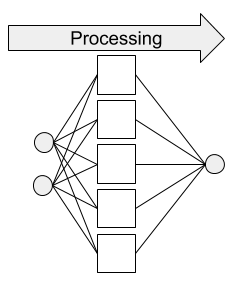
\includegraphics[width=0.25\textwidth]{sections/chapters/Chapter6/Images/Neural_network.png}
        }
    \subcaptionbox[B]{Quantum circuit with re-uploading}[.4\textwidth][c]{
        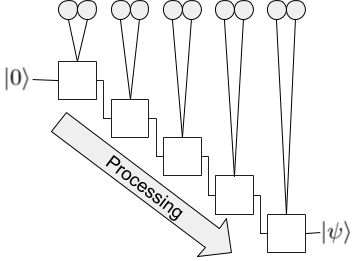
\includegraphics[width=0.5\textwidth]{sections/chapters/Chapter6/Images/Quantum_scheme.png}
        }
    \caption{
        Schemes of a one layer neural network and a single-qubit quantum circuit with data re-uploading.
        In the neural network the data is uploaded in each neuron of the hidden layer, hence data is 
        \textit{re-uploaded} multiple times.
        In a similar way the data is introduced classically numerous times in the circuit.
        The key difference between the two architectures is that each neuron of a neural network processes the 
        data in parallel and simultaneously, whereas the single-qubit quantum circuit with data re-uploading 
        processes the data sequentially.}
\label{Fig:schemes}
\end{figure}

In a single-qubit quantum circuit with data re-uploading, data is introduced as a rotation of the qubit.
Since every unitary can be expressed as the product of three rotation gates, we can define the angles as a linear
combination of weights and coordinates of the data\footnote[1]{Just like in a neuron of neural network.}.

\begin{equation}
    U(\bm{\phi}) = R_Z(\phi_1) R_Y(\phi_2) R_Z(\phi_3)
\label{}
\end{equation}

For instance, if data is 3-dimensional $\bm{x} = (x_1, x_2, x_3)$:

\begin{align}
    \phi_1 &= x_1 \cdot w_1 + b_1 \\
    \phi_2 &= x_2 \cdot w_2 + b_2 \\
    \phi_3 &= x_3 \cdot w_3 + b_3 \\
\end{align}

If data has a dimension greater than 3, we will need more than one unitary to encode a datapoint.
In general, if data has dimension \textit{d} we will need \(\left\lfloor \frac{d}{3} \right\rceil\) unitaries.
Each repetition of this \(\left\lfloor \frac{d}{3} \right\rceil\) unitaries to encode the data constitutes 
one layer of the architectures.

\begin{figure}
    \centering
    \begin{quantikz}
        \lstick{$\ket{0}$} &&& \gate{U(\phi_1, x)} 
        \gategroup[1,steps=1, style={dashed,rounded corners,fill=blue!20,inner xsep=6pt}, background, label style={label
        position=below, yshift=-0.4cm}]{L(1)} 
        &&& \ \ldots \ &&& \gate{U(\phi_N, x)} 
        \gategroup[1,steps=1, style={dashed,rounded corners,fill=blue!20,inner xsep=6pt}, background, label style={label
        position=below, yshift=-0.4cm}]{L(N)}
        &&& \meter{}
    \end{quantikz}
    \caption{The quantum circuit is divided into layers L(i), which constitutes the building blocks of this 
    architecture.}
\end{figure}

\end{comment}



    \clearpage
    % !TeX program = pdflatex
% !TeX root = ../main.tex

%*******************************************************
% Bibliografia
%*******************************************************
\cleardoublepage

\printbibliography
\end{document}